%\documentclass[draftclsnofoot,onecolumn]{IEEEtran}
\documentclass[3p]{elsarticle}
\usepackage{tipa}
\usepackage{amsmath}%math
\usepackage{amsthm}%proof
\usepackage{xcolor}%color
\usepackage{bm}
\usepackage{graphicx}
\usepackage{booktabs}
\usepackage{textcomp}
\usepackage[colorlinks,linkcolor=black,anchorcolor=black,citecolor=black]{hyperref}
\usepackage{amsfonts,amssymb}
\usepackage{color,soul}
\theoremstyle{plain}
\newtheorem{myas}{Assumption}
\newtheorem{mydef}{Definition}
\newtheorem{mylem}{Lemma}
\newtheorem{mythm}{Theorem}

%\theoremstyle{remark}
\theoremstyle{remark}
\newtheorem{myrem}{Remark}

\begin{document}
\begin{frontmatter}
\title{Dual Terminal Sliding Mode Control Design For Rigid Robotic Manipulator}
\author{Zhiqiang Ma}
\author{Guanghui Sun\corref{cor1}}
\ead{guanghuisun@hit.edu.cn}
\cortext[cor1]{Corresponding author}
\address{Research Institute of Intelligent Control and Systems, Harbin Institute of Technology, Harbin 150001, China}

\begin{abstract}
This paper proposes a dual terminal sliding mode control scheme for tracking tasks of rigid robotic manipulators. \textcolor{red}{As a significant novelty, the presented design technique integrates the individual sliding mode  surfaces to achieve the finite time convergence of tracking errors utilizing specially designed construct, and accordingly the convergence time is easily obtained due to the integral design. The underactuated issue and input limitation are specially considered in this paper, i.e., the underactuated issue is solved by introducing the hierarchical methodology into the basic dual sliding mode controller. The proposed method can easily combine with the adaptive technique to  eliminate the adverse effect caused by the input limitation in the rigorous stability analysis.} These newly proposed methods also have the characteristics of nonsingularity and chattering suppression, and the effectiveness and high efficiency are verified by stabilizing the motions of the overhead crane and the tracking tasks of the rigid robotic manipulator. Simulation results validate the theoretical analyses about the proposed method.
\end{abstract}
\begin{keyword}
Finite time control; Robotic manipulator control; Terminal sliding mode control; Input limitation; Stability analysis
\end{keyword}
\end{frontmatter}
\section{Introduction}
\textcolor{red}{Variable structure systems (VSS) are best known due to their insensitivity to parametric uncertainties~\cite{slotine1991applied}, and have been widely used in engineering applications, such as DC and DC converters~\cite{Tan2008General}, network control schemes~\cite{Hou2016}, aircrafts~\cite{Loza2015Sensor}, tethered satellite systems~\cite{Ma201667}, robotic manipulators~\cite{Beak2016A} and so on. As one important branch of the VSS, the sliding mode control (SMC) has become a popular solution to different kinds of control and signal process issues in recent years~\cite{zhao2015nonlinear,zhang2015attitude}. Meza-S{\'a}nchez et al. applied the second-order SMC scheme to a 3-DOF helicopter prototype based on the experimental test bed~\cite{meza2015output}. Zheng et al. implemented the SMC law to eliminate the bad effect of the input quantization in the coding and decoding process~\cite{zheng2016sliding}. Guzman et al. investigated the SMC application in a power factor rectifier with the constant switching frequency~\cite{guzman2016sliding}. Said et al. designed a robust adaptive sliding mode method to ensure the asymptotically stability of a boost converter~\cite{oucheriah2013pwm}. Roughly speaking, the SMC scheme is competent for normal scientific missions, due to its insensitivity to parametric uncertainties and external disturbances, however, there still exist some obstacles, such as noncontinuous switching inputs in high frequency and low convergence speed of the tracking errors~\cite{boiko2013chattering,lee2009chattering}, preventing it from being utilized in some high-precision engineering applications~\cite{fridman2011sliding}.}

\textcolor{red}{For alleviating the mentioned bad effects, many scientific researchers have presented remarkable achievements to promote the performance of SMC in last decade~\cite{zong2013quasi,santiesteban2013time,mu2015continuous,evangelista2013lyapunov,gonzalez2014chattering,dadras2012fractional,zhao2013output}. Among these methods, the high-order SMC and super-twisting SMC work well in reducing the chattering to generate continuous inputs~\cite{castillo2015higher,palosz2015laser,edwards2016adaptive,zhao2015finite,liu2015second}. Besides the issue on repressing the chattering, the fast convergence of the SMC scheme becomes a hot subject recently. The normal linear SMC completes the stabilization of the system dynamics in two steps. In the first step, the control inputs drive the system states onto the prescript sliding mode  surfaces, and this stage is also called the reaching phase. Then the sliding mode dynamics function to drive the system states to the origins along the ideal surfaces in the second step, which is usually known as the sliding phase. The reaching phase usually requires the states to reach the ideal sliding mode surfaces in finite time, and suitably selected Lyapunov function and control parameters may accelerate this process; the sliding phase is related to the designed ideal sliding mode  surfaces closely, and trivial design techniques can guarantee the asymptotically stability of the reduced system~\cite{mu2016switching}. To achieve a fast convergence in the sliding phase, the terminal sliding mode (TSM) control is developed based on the finite time control theory~\cite{haimo1986finite,bhat1997finite}, and compared with the SMC design mentioned above, the most significant contributions of the TSM concept are introducing the finite time convergence to the sliding phase to complete the global finite time convergence~\cite{mu2016switching}. Moreover, the terminal SMC schemes have been utilized to achieve the high precise control, i.e., in~\cite{li2015robust}, an adaptive TSM controller regulated a $2$-link robotic manipulator to track the variable signals. Feng et al. stated a novel Lagrangian dynamic expression for the the rigid robot, and applied the global TSM control law to manipulate the robotic dynamics ~\cite{feng2002non}. In~\cite{kamal2016continuous}, Kamal addressed a continuous homogeneous sliding mode algorithm for a perturbed second-order plant, and the algorithm could be regarded as a combination of TSM and super-twisting sliding mode schemes.}

\textcolor{red}{Notably, the conventional TSM surface design techniques are similar, since the surfaces are all designed for the single variable based on the finite time stability theory, in other words, only the individual variable and its derivative are concerned on by most designers~\cite{mu2016switching}. This nature makes the TSM controller become an individual control subsystem, which leads to the complicity of global convergence time in some extent. In this paper, an integral sliding mode  surface design technique breaks the barriers mentioned above, and the novel surface includes two designed variables to guarantee the integral finite time convergence. Moreover, nonsingularity of the TSM control scheme, chattering suppressions, underactuated applications and input limitations are also considered in the controller design.}

\textcolor{red}{In this paper, the dual TSM (DTSM) control scheme is proposed for a class of second-order nonlinear systems with disturbances and uncertainties. The novel DTSM surface is exploited to achieve the finite time convergence, and the reaching and sliding times can both be calculated directly. For coping with the underacutated issue, cooperating with the hierarchical sliding mode  surface design methodology, we combine the hierarchical SMC scheme with the DTSM controller to develop a hierarchical dual TSM (HDTSM) control law to ensure the rigorous stability analyses. A modified DTSM (MDTSM) control scheme is presented to regulate the motion of the $n$-link robotic manipulators, and the case subjected to input limitations is also taken into consideration. The remained paper is organized as follows: Section~\ref{sec:2} introduces the DTSM controller, and the finite time convergence is discussed. Furthermore, we provide the DTSM control scheme with extra design parameters to obtain the MDTSM controller, which performs better in theoretical analyses; for stabilizing underactuated systems, the HDTSM controller design is also developed in this section. In Section~\ref{sec:3}, the MDTSM control law is applied to the motion control system of the $n$-link robotic  manipulator, and the stability analyses are also carried out. Section~\ref{sec:4} exhibits the simulation results, and finally the conclusion is assigned in Section~\ref{sec:5}.}
\section{Dual terminal SMC}\label{sec:2}
Consider a nominal second-order nonlinear system:
\begin{align}
\begin{split}
\dot x_1 &= x_2\\
\dot x_2 &= f_1(\bm x,t)+g_1(\bm x,t)+b_1(\bm x,t)u_1\\
\dot x_3 &= x_4\\
\dot x_4 &= f_2(\bm x,t)+g_2(\bm x,t)+b_2(\bm x,t)u_2,\label{eq:second-order system}
\end{split}
\end{align}
where $\bm x = [x_1,x_2,x_3,x_4]^T$ is the system state vector ; $f(\bm x,t)$ and $b(\bm x,t)\neq 0$ are smooth nonlinear functions with respect to $\bm x$ and $t$; $u_i$, $i=1,2$ stands for the system input; $g_i(\bm x,t)$, $i=1,2$  is defined as the bounded nonlinear function which satisfies $\Vert g_i(\bm x,t)\Vert\le l_i$, $l_i>0, i=1,2$, meaning uncertainties and disturbances. For the system mentioned above, we can design the desired DTSM surface as:
\begin{align}
\bm s = [s_1,s_2]^T,
\end{align}
where
\begin{align}
\begin{split}
s_1 &= x_2+\vert x_1\vert^{\alpha} sgn(x_1)+x_1^3-x_3\\
s_2 &= x_4+\vert x_3\vert^{\alpha} sgn(x_3)+x_3^3+x_1.\label{eq:dual sliding mode  surface}
\end{split}
\end{align}
\textcolor{red}{$sgn(x)$ is the sign function, and $0<\alpha<1$ is a positive scalar. For the sake of simplicity, the symbol $t$ is usually omitted in this paper, and it will appear once the derivation concerns for the factor of the time strictly, i.e., the desired sliding mode  surface $\bm s(t)$ is often abbreviated as $\bm s$.}

There exist two lemmas facilitating the derivation of the finite time convergence about the DTSM controller.
\begin{mylem}
As described in~\cite{moulay2006finite}, it's assumed that the continuous function $V$ is positive definite, satisfying following conditions:
\begin{align}
\dot V\le -dV^\beta\quad\forall t\ge t_0, V(t_0)\ge 0,
\end{align}
where $d$ is a positive scalar, and $0<\beta<1$. Then the function $V$ converges to the origin for any given $t_0$, and typically the finite convergence time $t_r$ can be given as follows:
\begin{align}
t_r \le t_0+\frac{V^{1-\beta}(t_0)}{d(1-\beta)}.
\end{align}\label{lemma:1}
\end{mylem}
\begin{mylem}
Consider a second-order system:
\begin{align}
\begin{split}
\dot x_1&=-\vert x_1\vert^\alpha sgn(x_1)-x_1^3+x_2\\
\dot x_2&=-\vert x_2\vert^\alpha sgn(x_3)-x_2^3-x_1,\label{eq:normal sliding mode  surface}
\end{split}
\end{align}
and one can select the function $V = \frac{x_1^2+x_2^2}{2}$ to obtain the finite convergence time as follows~\cite{moulay2006finite}:
%since $\vert x\vert-x^\alpha+\vert x\vert \ge 0,0<\alpha<1$
\begin{align}
%t_s\le t_0+\frac{2(x_1^2+x_2^2)^{1-\alpha}}{1-\alpha}
t_s\le t_0+\frac{(2V(t_0))^{\frac{1-\alpha}{2}}}{1-\alpha},
\end{align}
where the definitions of  $t_s$, $t_0$, $\alpha$ are similar to Lemma \ref{lemma:1}. Introducing the scalar $d$ into the Eq.~(\ref{eq:normal sliding mode  surface}) obtains:
\begin{align}
\dot x_1&=-d(\vert x_1\vert^\alpha sgn(x_1)-x_1^3+x_2)\\
\dot x_2&=-d(\vert x_2\vert^\alpha sgn(x_2)-x_2^3-x_1),\label{eq:more normal sliding mode  surface}
\end{align}
the convergence time of which is
\begin{align}
t_s\le t_0+\frac{(2V(t_0))^{\frac{1-\alpha}{2}}}{d(1-\alpha)}.
\end{align}\label{lemma:2}
\end{mylem}
\textcolor{red}{For stabilization of the second-order system shown as~Eq.~(\ref{eq:second-order system}), DTSM control inputs are stated according the following theorem.}
\begin{mythm}\label{theorem:1}DTSM Controller Design. The states of the system~(\ref{eq:second-order system}) will converge to origins along the surface $\bm s=0$ in finite time, if the inputs are designed as
\begin{align}
\begin{split}
u_1 &= -b_1^{-1}(\bm x)(f_1(\bm x)+\alpha\vert x_1\vert^{\alpha-1}x_2+3x_1^2x_2-x_4+k_1sgn(s_1))\\
u_2 &= -b_2^{-1}(\bm x)(f_2(\bm x)+\alpha\vert x_3\vert^{\alpha-1}x_4+3x_3^2x_4+x_2+k_2sgn(s_2)),\label{eq:DSM input}
\end{split}
\end{align}
where $k_i = l_i+\eta_i$, $i=1,2$; $\eta_i>0$ is a positive scalar value.
\end{mythm}
\begin{proof}
\textcolor{red}{For the system~(\ref{eq:second-order system}) with the sliding mode  surface~(\ref{eq:dual sliding mode  surface}), according to the equivalent control technique and the sliding mode  surface reaching condition~\cite{Arie1993sliding}, the inputs can be designed as
\begin{align}\begin{split}
u_1 &= u_{eq1}+u_{sw1}\\
u_2 &= u_{eq2}+u_{sw2}\notag
\end{split}\end{align}
where
\begin{align}\begin{split}
u_{eq1} &= -b_1^{-1}(\bm x)(f_1(\bm x)+\alpha\vert x_1\vert^{\alpha-1}x_2+3x_1^2x_2-x_4)\\
u_{eq2} &= -b_2^{-1}(\bm x)(f_2(\bm x)+\alpha\vert x_3\vert^{\alpha-1}x_4+3x_3^2x_4+x_2)\notag
\end{split}\end{align}
are the equivalent control inputs, which ensure $\dot s_1 = 0$ and $\dot s_2=0$ with $u_i = u_{eqi}$, $i=1,2$. The switching inputs can be selected as $u_{swi}=-b_i^{-1}k_isgn(s_i)$, $i=1,2$ to guarantee the finite time reaching conditions of the sliding mode  surface.}

Consider the Lyapunov function $V=\frac{1}{2}{\bm s}^T\bm s$, which has
\begin{align}
\begin{split}
\dot V &= {\bm s}^T\dot{\bm  s}\\
&=s_1\dot s_1+s_2\dot s_2\\
&=s_1(f_1(\bm x)+g_1(\bm x)+b_1(\bm x)u_1+\alpha\vert x_1\vert^{\alpha-1}x_2+3x_1^2x_2-x_4)\\
&\quad +s_2(f_2(\bm x)+g_2(\bm x)+b_2(\bm x)u_2+\alpha\vert x_3\vert^{\alpha-1}x_4+3x_3^2x_4+x_2).\label{eq:V_1}
\end{split}
\end{align}
Substituting inputs (\ref{eq:DSM input}) in~Eq.~(\ref{eq:V_1}) yields
\begin{align*}
\dot V &= s_1(-k_1sgn(s_1)+g_1(\bm x))+s_2(-k_2sgn(s_2)+g_2(\bm x))\\
&= -\eta_1s_1sgn(s_1)-\eta_2s_2sgn(s_2)+(g_1(\bm x)s_1 - l_1s_1sgn(s_1))+(g_2(\bm x)s_2 - l_2s_2sgn(s_2))\\
&= -\eta_1\vert s_1\vert-\eta_2\vert s_2\vert+(g_1(\bm x)s_1 - l_1\vert s_1\vert)+(g_2(\bm x)s_2 - l_2\vert s_2\vert)\\
&\le - \min(\eta_1,\eta_2)(\vert s_1\vert+\vert s_2\vert)\\
&\le -\min(\eta_1,\eta_2)({\bm s}^T\bm s)^\frac{1}{2}\\
&\le -\sqrt{2}\min(\eta_1,\eta_2)V^\frac{1}{2}\le 0.
\end{align*}
Hence, the system (\ref{eq:second-order system}) converges to the desired sliding mode  surface (\ref{eq:dual sliding mode  surface}), and incidentally the convergence time can be obtained according to the finite time convergence theory. Once the system (\ref{eq:second-order system}) satisfies $\bm s = \bm 0$, the entire system states will be handled by the reduced system:
\begin{align}
  \begin{split}
\dot x_1&=-\vert x_1\vert^\alpha sgn(x_1)-x_1^3+x_3\\
\dot x_3&=-\vert x_3\vert^\alpha sgn(x_3)-x_3^3-x_1\label{eq:reduced system}
\end{split}
\end{align}
\textcolor{red}{The total convergence time can be calculated by dividing the convergence into two phases with respect to the relation of the system states and the DTSM surface, namely, the reaching phase and the sliding phase. Hence, according to Lemma \ref{lemma:2}, the theoretical total finite convergence time $t_f$ can be calculated from:
\begin{align}
t_f = \underbrace{t_0+\frac{\sqrt{2}V^{\frac{1}{2}}(t_0)}{\min(\eta_1,\eta_2)}}_{t_r}+\underbrace{\frac{(2\hat V(t_r))^{\frac{1-\alpha}{2}}}{1-\alpha}}_{t_s}<\infty,
\end{align}
where $\hat V = \frac{x_1^2+x_3^2}{2}$ is the Lyapunov function selected for the reduced system~(\ref{eq:reduced system}). $t_r$ and $t_s$ stand for the reaching time and the sliding time, respectively. This completes the proof.}
\end{proof}
On the basis of Theorem \ref{theorem:1}, we proceed to develop the parameters in the sliding mode  surface design to improve the performance of the reaching phase, and furthermore this modified method makes the design process more flexible. Consider the system~(\ref{eq:second-order system}) with the surface $\bm s = [s_1,s_2]^T$ described by following expressions:
\begin{align}
\begin{split}
s_1 &= x_2+\gamma(\vert x_1\vert^{\alpha} sgn(x_1)+x_1^3)-\lambda x_3\\
s_2 &= x_4+\gamma(\vert x_3\vert^{\alpha} sgn(x_3)+x_3^3)+\lambda x_1,\label{eq:modified dual sliding mode  surface}
\end{split}
\end{align}
where $\gamma$ is a positive constant and $\lambda\in R$ is a design parameter. Accordingly, the modified DTSM control inputs are formed in the following theorem.
\begin{mythm}\label{theorem:2}Modified DTSM Controller Design.
The second-order system (\ref{eq:second-order system}) will reach the desired sliding mode  surface $\bm s = \bm 0$ shown in~Eq.~(\ref{eq:modified dual sliding mode  surface}) in finite time, and then the system states will converge to origins along the surface $\bm s=\bm 0$ in finite time, if the inputs are expressed as
\begin{align}
\begin{split}
u_1 &= -b_1^{-1}(\bm x)(f_1(\bm x)+\gamma\alpha\vert x_1\vert^{\alpha-1}x_2+3\gamma x_1^2x_2-\lambda x_4+k_1sgn(s_1))\\
u_2 &= -b_2^{-1}(\bm x)(f_2(\bm x)+\gamma\alpha\vert x_3\vert^{\alpha-1}x_4+3\gamma x_3^2x_4+\lambda x_2+k_2sgn(s_2)),\label{eq:modified input}
\end{split}
\end{align}
where $k_i = l_i+\eta_i$, $i=1,2$; $\eta_i>0$ is a positive scalar. The total finite convergence time is given out directly:
\begin{align}
t_f = \underbrace{t_0+\frac{\sqrt{2}V^{\frac{1}{2}}(t_0)}{\min(\eta_1,\eta_2)}}_{t_r}+\underbrace{\frac{(2\hat V(t_r))^{\frac{1-\alpha}{2}}}{\gamma(1-\alpha)}}_{t_s}<\infty,\label{eq:total convergence time}
\end{align}
\end{mythm}
\begin{proof}
The proof is similar to Theorem \ref{theorem:1}, hence it's omitted here.
\end{proof}
In the MDTSM control scheme, the performances of the reaching and sliding phases can benefit from suitably selected $\lambda$ and $\gamma$ analytically. The establishment of $V(t_0)$ depends on $\lambda$, if the state $\bm x(t_0)$ has been fixed. Exactly, $\lambda$ affects the reaching distance between $V(t_0)$ and $V(t_r)$, and normally $V(t_r)$ stands for the reaching status at $t_r$, namely, $V=\bm s^T\bm s = \bm 0,\forall t\ge t_r$. $\eta$ is defined as the reaching speed, because a suitable $\eta$ can adjust the reaching time as desired in some extent. Hence, $\lambda$ cooperates with $\eta$ to manage the reaching phase dynamics, and similarly the parameter $\gamma$ determine the convergence speed of the sliding phase dynamics.
\begin{myrem}
For the proposed designs, the parameter $\gamma$ may be defined as different scalars $\gamma_1$ and $\gamma_2$ for $u_1$ and $u_2$ respectively, such that one can produce the total convergence time as:
\begin{align}
t_f = \underbrace{t_0+\frac{\sqrt{2}V^{\frac{1}{2}}(t_0)}{\min(\eta_1,\eta_2)}}_{t_r}+\underbrace{\frac{(2\hat V(t_r))^{\frac{1-\alpha}{2}}}{\min(\gamma_1,\gamma_2)(1-\alpha)}}_{t_s}<\infty.\label{eq:normal total convergence time}
\end{align}
\end{myrem}
\subsection{Nonsingular MDTSM controller design}

The finite time convergence of the MDTSM controller has been verified clearly, but similar to the conventional TSM control scheme, there exists another obstacle in the design mentioned above, i.e., the issue of the singularity in control inputs. Essentially, the singularity occurs in Eq.~(\ref{eq:modified input}) when $x_1=0$ but $x_2\neq 0$ in $u_1$ (the phenomena happens to $u_2$ under the same condition). To cope with the singularity, the nonsingular MDTSM control scheme is presented after introducing the analytical technique into the MDTSM controller based on the following lemma~\cite{feng2013nonsingular}.
\begin{mylem}\label{lemma:3}
Considering the second-order system (\ref{eq:second-order system}), the TSM surfaces are designed as:
\begin{align*}
s_1 &= x_2+\gamma_1\vert x_1\vert^{\alpha_1}sgn(x_1)\\
s_2 &= x_4+\gamma_2\vert x_3\vert^{\alpha_2}sgn(x_3),
\end{align*}
and nonsingular inputs can be given out directly as follows:
\begin{align*}
u_1 &= b^{-1}_1(\bm x)(-f_1(\bm x)+sat(u_{f1},u_{s1})-k_1sgn(s_1))\\
u_2 &= b^{-1}_2(\bm x)(-f_2(\bm x)+sat(u_{f2},u_{s2})-k_2sgn(s_2)),
\end{align*}
in which
\begin{align*}
u_{f1}&=-\gamma_1\alpha_1\vert x_1\vert^{\alpha_1-1}x_2\\
u_{f2}&=-\gamma_2\alpha_2\vert x_3\vert^{\alpha_2-1}x_4,
\end{align*}
$sat(u_f,u_s)$ is a saturation function:
\begin{align}
sat(u_f,u_s)=
\begin{cases}
u_s\quad &u_f\ge u_s\\
u_f\quad &-u_s\le u_f< u_s\\
-u_s\quad &u_f\le -u_s\label{eq:saturation}
\end{cases},
\end{align}
with $u_s>0$. Adopting the control scheme mentioned above, the system~(\ref{eq:second-order system}) will be stabilized in finite time without any singularity occurring during the regulation process.
\end{mylem}
\begin{mythm}\label{theorem:3}
Consider a second-order system (\ref{eq:second-order system}), and for eliminating the singularity, the inputs are selected to complete the nonsingular MDTSM control scheme. Introducing the saturation terms~(\ref{eq:saturation}) into the original inputs yields:
\begin{align}
u_1 &= -b_1^{-1}(\bm x)(f_1(\bm x)-sat(u_{f1},u_{s1})+3\gamma x_1^2x_2-\lambda x_4+k_1sgn(s_1))\\
u_2 &= -b_2^{-1}(\bm x)(f_2(\bm x)-sat(u_{f2},u_{s2})+3\gamma x_3^2x_4+\lambda x_2+k_2sgn(s_2)),\label{eq:nonsingular modified input}
\end{align}
and one can obtain a nonsingular solution to the stabilization of the system~(\ref{eq:second-order system}), providing the finite time convergence using MDTSM control technique.
\end{mythm}
\begin{proof}
The proof is similar to the graphical analysis mentioned in~\cite{feng2013nonsingular}, and omitted here.
\end{proof}
\subsection{MDTSM controller design for systems subjected to input limitations}
\textcolor{red}{
Besides singularity issue, in practice, the control input can not be very large due to the input limitation, such as the tension limitation in the deployment of the tethered satellite system~\cite{Ma201667}, and hence it is meaningful to adapt the proposed controllers for the system subjected to the input limitation. Consider a nominal second-order system subjected to the input limitation:
\begin{align}
\begin{split}
\dot x_1 &= x_2\\
\dot x_2 &= f_1(\bm x,t)+g_1(\bm x,t)+b_1(\bm x,t)f_b(u_1)\\
\dot x_3 &= x_4\\
\dot x_4 &= f_2(\bm x,t)+g_2(\bm x,t)+b_2(\bm x,t)f_b(u_2),\label{eq:second-order system subjected to limitation}
\end{split}
\end{align}
where $f_b(u) = R(u)u$ is a bounded function, which owns the properties as follows:
\begin{align}\begin{split}
  R(u)=\begin{cases}
  u_{max}/u &u>u_{max}\\
  1&u_{min}\le u\le u_{max}\\
  u_{min}/u& u<u_{min}.
\end{cases}\end{split}
\end{align}
\begin{myas}~\cite{Ma201667}\label{myas:1}
For guaranteeing $0<R(u)\le 1$, $u_{max}$ and $u_{min}$ satisfy $u_{min}<0<u_{max}$. The external disturbance $g_i(\bm x,t)$, inputs $u_i$, $i=1,2$ and system state variables are all bounded, accordingly,
\begin{align}\begin{split}
  \varpi_1 &\ge \Vert f_1(\bm x)+\gamma\alpha\vert x_1\vert^{\alpha-1}x_2+3\gamma x_1^2x_2-\lambda x_4+g_1(\bm x)\Vert\\
  \varpi_2 &\ge \Vert f_2(\bm x)+\gamma\alpha\vert x_3\vert^{\alpha-1}x_4+3\gamma x_3^2x_4+\lambda x_2+g_2(\bm x)\Vert\\
  0&<\varphi\le R(u) \le 1
\end{split}\end{align}
\end{myas}
Thanks to the above assumption, we can give out the adaptive DTSM controller.
\begin{mythm}\label{thm:4}
Considering the nominal second-order system subjected to the input limitation~(\ref{eq:second-order system subjected to limitation}), the inputs $u_i$,$i=1,2$ can be designed as
\begin{align}
  u_i &= -\varpi_i\nu_i\omega_i b_i^{-1}sgn(s_i)\\
  \dot\omega_i&= \varpi_i\nu_i\varphi_i e^{-2\varphi_i^{-1}\omega_i^{-1}}\vert s_i\vert
\end{align}
with $\nu_i>1$ and $\omega_i(0)>0$, such that the trajectories of the system states can converge to the sliding mode  surfaces in Eq.~(\ref{eq:modified dual sliding mode  surface}).
\end{mythm}
\begin{proof}
Consider the Lyapunov function
$$V=\frac{1}{2}\bm s^T\bm s+\frac{1}{2}v_1^2+\frac{1}{2}v_2^2$$
with
$$v_i = \omega_ie^{\varphi_i^{-1}\omega_i^{-1}}$$
and hence we can proceed to obtain the derivative of the Lyapunov function
\begin{align}\begin{split}
\dot V &=s_1\dot s_1+s_2\dot s_2+v_1\dot v_1+v_2\dot v_2\\
&=s_1(f_1(\bm x)+\gamma\alpha\vert x_1\vert^{\alpha-1}x_2+3\gamma x_1^2x_2-\lambda x_4+g_1(\bm x)+b_1(\bm x)u_1)\\
&\quad +s_2(f_2(\bm x)+\gamma\alpha\vert x_3\vert^{\alpha-1}x_4+3\gamma x_3^2x_4+\lambda x_2+g_2(\bm x)+b_2(\bm x)u_2)\\
&\quad+\varpi_1\nu_1(\omega_1-1)\vert s_1\vert+\varpi_2\nu_2(\omega_2-1)\vert s_2\vert\\
&\le \varpi_1\vert s_1\vert+\varpi_2\vert s_2\vert-\varpi_1\nu_1\omega_1\vert s_1\vert-\varpi_2\nu_2\omega_2\vert s_2\vert\\
&\quad + \varpi_1\nu_1(\omega_1-1)\vert s_1\vert+\varpi_2\nu_2(\omega_2-1)\vert s_2\vert\\
&\le -\varpi_1(\nu_1-1)\vert s_1\vert-\varpi_2(\nu_2-1)\vert s_2\vert\le 0\label{V linmitation}
\end{split}\end{align}
$\dot V$ is therefore negative semi-definite while $V_1$ is positive definite. Since  $s_i$ is bounded according to assumption~\ref{myas:1}, we can have $\lim_{t\to\infty}V<\infty$ and proceed to deduce the integration of inequality~(\ref{V linmitation}) to obtain following results
\begin{align}\begin{split}
V(0)&\ge V(t)+\int_0^t(\nu_1-1)\varpi_1\vert s_1(\varsigma)\vert+(\nu_2-1)\varpi_2\vert s_2(\varsigma)\vert d\varsigma\\
&\ge\int_0^t(\nu_1-1)\varpi_1\vert s_1(\varsigma)\vert+(\nu_2-1)\varpi_2\vert s_2(\varsigma)\vert d\varsigma.
\end{split}\end{align}
Hence we can conclude that the sliding dynamics are asymptotically stable in the light of Barbalat lemma. Here the proof completes, and the system states can converge to origins by referring to the analyses in Theorem~\ref{theorem:1}.
\end{proof}
}
\subsection{MDTSM controller design for underactuated systems}
When the input $u_1$ equals to $u_2$ in system~(\ref{eq:second-order system}), the number of the inputs is fewer than the degree of the freedom, which leads to the underactuated issue. These underactuated systems are ubiquitous and welcomed in the scientific and engineering fields, because fewer actuators may decrease the mass and save the energy. Cooperating with the hierarchical sliding mode methodology, the presented MDTSM control law can stabilize this kind of systems~\cite{wang2004design}. Here, we provide the hierarchical MDTSM controller directly.
\begin{mythm}
Consider the nonlinear system described as:
\begin{align}
\begin{split}
&\dot x_1 = x_2\\
&\dot x_2 = f_1(\bm x) + g_1(\bm x)+b_1(\bm x)u\\
&\dot x_3 = x_4\\
&\dot x_4 = f_2(\bm x) + g_2(\bm x)+b_2(\bm x)u,\label{eq:underactuated system}
\end{split}
\end{align}
where the conditions of variables are same to the system~(\ref{eq:second-order system}). Construct the sliding mode  surfaces as:
\begin{align}
S = c_1s_1+c_2s_2,
\end{align}
where $c_1$ and $c_2$ are suitable positive constants, and $s_1$ and $s_2$ have been defined in Eq.~(\ref{eq:dual sliding mode  surface}). Adopting the equivalent control design method deduces the individual equivalent inputs:
\begin{align}
\begin{split}
&u_{eq1} = -b_1^{-1}(\bm x)(f_1(\bm x)+\gamma\alpha\vert x_1\vert^{\alpha-1}x_2+3\gamma x_1^2x_2-\lambda x_4)\\
&u_{eq2} = -b_2^{-1}(\bm x)(f_2(\bm x)+\gamma\alpha\vert x_3\vert^{\alpha-1}x_4+3\gamma x_3^2x_4+\lambda x_2),
\end{split}
\end{align}
and the control law $u$ has the following formula:
\begin{align}
u = (c_1b_1(\bm x)+c_2b_2(\bm x))^{-1}(c_1b_1(\bm x)u_{eq1}+c_2b_2(\bm x)u_{eq2}-\eta_u sign(S)-k_u S)\label{eq:underactuated input}
\end{align}
which can stabilize the underactuated system~(\ref{eq:underactuated system}) as desired in finite time.
\end{mythm}
\begin{proof}
Select a Lyapunov function candidate $V=\frac{1}{2}S^2$, and differentiate it with respect to time $t$:
\begin{align}
\begin{split}
\dot V &= S\dot S\\ &= S(c_1\dot s_1+c_2\dot s_2)\\
&=S(c_1(f_1(\bm x)+g_1(\bm x)+b_1(\bm x)u+\gamma\alpha\vert x_1\vert^{\alpha-1}x_2+3\gamma x_1^2x_2-\lambda x_4)\\
&\quad+c_2(f_2(\bm x)+g_2(\bm x)+b_2(\bm x)u+\gamma\alpha\vert x_3\vert^{\alpha-1}x_4+3\gamma x_3^2x_4+\lambda x_2))\\
&=S(c_1(f_1(\bm x)+g_1(\bm x)+\gamma\alpha\vert x_1\vert^{\alpha-1}x_2+3\gamma x_1^2x_2-\lambda x_4)\\
&\quad+c_2(f_2(\bm x)+g_2(\bm x)+\gamma\alpha\vert x_3\vert^{\alpha-1}x_4+3\gamma x_3^2x_4+\lambda x_2)+(c_1b_1(\bm x)+c_2b_2(\bm x))u).\label{eq:underactuated Lyapunov}
\end{split}
\end{align}
Substituting the input~(\ref{eq:underactuated input}) into Eq.~(\ref{eq:underactuated Lyapunov}) leads to
\begin{align}
\begin{split}
\dot V &= S(c_1(f_1(\bm x)+g_1(\bm x)+\gamma\alpha\vert x_1\vert^{\alpha-1}x_2+3\gamma x_1^2x_2-\lambda x_4)\\
&\quad+c_2(f_2(\bm x)+g_2(\bm x)+\gamma\alpha\vert x_3\vert^{\alpha-1}x_4+3\gamma x_3^2x_4+\lambda x_2)\\
&\quad+(c_1b_1(\bm x)u_{eq1}+c_2b_2(\bm x)u_{eq2}-\eta_u sign(S)-k_u S))\\
&= S(c_1g_1(\bm x)+c_2g_2(\bm x)-\eta_u sign(S)-k_u S)\\
&\le -(\eta_u -\vert c_1g_1(\bm x)+c_2g_2(\bm x)\vert)\vert S\vert-k_u S^2.
\end{split}
\end{align}
As $\vert g_i(\bm x)\vert<l_i$ exists, a big enough $\eta_u$ may be chosen to guarantee the reaching condition of the surface $S$. The proof of the stability of the desired sliding mode  surfaces $s_1$ and $s_2$ is same to the one in \cite{wang2004design}, and omitted here. This completes the proof.
\end{proof}
\section{MDTSM controller design for rigid manipulators}\label{sec:3}
In this section, the MDTSM controller designed for the stabilization of the rigid $n$-link robotic manipulator is discussed. Firstly, we consider the $2$-link robotic manipulator dynamics~\cite{feng2002non}:
\begin{align}
M(\bm q)\ddot {\bm q}+C(\bm q,\dot {\bm q})+g(\bm q)= \bm\tau+{\bm d},\label{eq:lagrangian system}
\end{align}
where $\bm q\in R^{2} $ is the joint angular position vector; ${M(\bm q)}\in R^{2\times 2}$ is the inertia matrix; ${C(\bm q,\dot{\bm q})}\in R^{2\times 1}$ denotes Coriolis and centrifugal forces; ${g(\bm q)}\in R^{2\times 1}$ stands for the gravitational torque; $\bm{\tau}\in R^{2\times 1}$ is referred to as the joint torques; $\bm d\in R^{2\times 1}$ expresses the bounded disturbance vector. Normally, there exist some uncertainties in the manipulator, and the dynamic equations are revised as
\begin{align}
(M_0(\bm q)+\Delta {M(\bm q))\ddot {\bm q}}+({C_0(\bm q,\dot {\bm q})+\Delta C(\bm q,\dot {\bm q})})+g_0(\bm q)+\Delta g(\bm q)=\bm {\tau}+\bm{d},
\end{align}
where $M_0(\bm q)$, $C_0(\bm q,\dot {\bm q})$ and $g_0(\bm q)$ are the estimated terms, while $\Delta M_0(\bm q)$, $\Delta C_0(\bm q,\dot {\bm q})$, $\Delta g_0(\bm q)$ denotes the uncertainties in the manipulator dynamics. Particularly, the following assumptions exist to explain the bounded characteristics of the dynamics~\cite{feng2002non}:
\begin{align}
&\Vert M(\bm q)\Vert< \theta_0\notag\\
&\Vert C(\bm q,\dot {\bm q})\Vert< \phi_0+\phi_1\Vert\bm q\Vert+\phi_2\Vert\dot{\bm q}\Vert^2\notag\\
&\Vert g(\bm q)\Vert< \psi_0+\psi_1\Vert\bm q\notag\Vert\\
&\Vert \bm {\rho}\Vert< \mu_0+\mu_1\Vert\bm q\Vert+\mu_2\Vert\dot{\bm q}\Vert^2,\label{eq:manipulator uncertainty}
\end{align}
where $\bm {\rho} = -\Delta M(\bm q)-\Delta C(\bm q,\dot {\bm q})-\Delta g(\bm q)$, and $\theta_0$, $\phi_0$, $\phi_1$, $\phi_2$, $\psi_0$, $\psi_1$, $\mu_0$, $\mu_1$, $\mu_2$ are positive constants.\par
Select $\bm q_d$ as the desired state vector of the manipulator dynamics~(\ref{eq:lagrangian system}), and the derivative of $\bm q_d$ is designated as $\dot {\bm q}_d$. Hence the state error is stated as:
\begin{align}
\bm \varepsilon = \bm q -\bm q_d.
\end{align}
With the purpose of simplifying the proceeding derivation, some symbol definitions for vector operation are presented in advance. For expressing the $n$-dimension vector including a sort of compound functions, the following symbol is introduced:
\begin{align*}
\lceil\bm h\bm p+\bm v\rfloor = (h_1p_1+v_1,h_2p_2+v_2,\ldots,h_np_n+v_n)^T.
\end{align*}
On the basis of the above results, one can design the DTSM controller for the $2$-link robotic manipulator by utilizing the following theorem.
\begin{mythm}\label{theorem:4}
For the rigid $2$-link manipulator~(\ref{eq:lagrangian system}), if the DTSM surface is selected as
\begin{align}
\bm s = \dot{\bm \varepsilon}+C_\gamma\lceil\bm{sgn}^\alpha(\bm \varepsilon)+\bm\varepsilon^3\rfloor+C_\lambda{\bm\varepsilon},\label{eq:lagrangian surface}
\end{align}
where
\begin{align}
\begin{split}
&C_\gamma=diag[\gamma_1,\gamma_2]\\
&C_\lambda=
\begin{pmatrix}
0 &-\lambda\\ \lambda &0
\end{pmatrix}\\
&{sgn}^\alpha(\varepsilon)=\vert\varepsilon\vert^\alpha sgn(\varepsilon),
\end{split}
\end{align}
furthermore, the corresponding input follows to stabilize the system~(\ref{eq:lagrangian system}) as desired in finite time.
\begin{align}
\begin{split}
\bm\tau &= \bm u_0+\bm u_1 +\bm u_2\\
\bm u_0 &= -M_0(\bm q)C_r\lceil\alpha\vert\bm\varepsilon\vert^{\alpha-1}\dot{\bm \varepsilon}+3\bm \varepsilon^2\dot{\bm \varepsilon}\rfloor-M_0(\bm q)C_\lambda\dot{\bm \varepsilon}\\
\bm u_1 &= M_0(\bm q)\ddot {\bm q}_d+C_0(\bm q,\dot {\bm q})+g_0(\bm q)\\
\bm u_2 &= -k\frac{(\bm s^TM_0^{-1}(\bm q))^T}{\Vert\bm s^TM_0^{-1}(\bm q)\Vert}.
\end{split}
\end{align}
in which $k>\mu_0+\mu_1\Vert\bm q\Vert+\mu_2\Vert\dot{\bm q}\Vert^2$, and it's assumed that the parameters $\mu_0$, $\mu_1$ and $\mu_2$ are known.
\end{mythm}
\begin{proof}
Select the Lyapunov function
\begin{align}
V=\frac{1}{2}\bm s^T\bm s,
\end{align}
the derivative of which is described as
\begin{align}
\begin{split}
\dot V &= \bm s^T\dot{\bm s}=\bm s^T(\ddot{\bm \varepsilon}+C_r\lceil\alpha\vert\bm\varepsilon\vert^{\alpha-1}\dot{\bm \varepsilon}+3\bm \varepsilon^2\dot{\bm \varepsilon}\rfloor+C_\lambda\dot{\bm \varepsilon})\\
&=\bm s^T(M_0^{-1}(\bm q)(-M_0(\bm q)\ddot {\bm q}_d-C_0(\bm q,\dot {\bm q})-g_0(\bm q)+\bm\tau+\bm\rho)\\
&\quad+C_r\lceil\alpha\vert\bm\varepsilon\vert^{\alpha-1}\dot{\bm \varepsilon}+3\bm \varepsilon^2\dot{\bm \varepsilon}\rfloor+C_\lambda\dot{\bm \varepsilon})\\
&=\bm s^T(M_0^{-1}(\bm q)(\bm u_0+\bm u_2+\bm\rho)+C_r\lceil\alpha\vert\bm\varepsilon\vert^{\alpha-1}\dot{\bm \varepsilon}+3\bm \varepsilon^2\dot{\bm \varepsilon}\rfloor+C_\lambda\dot{\bm \varepsilon})\\
&=\bm s^TM_0^{-1}(\bm q)(-k\frac{(\bm s^TM_0^{-1}(\bm q))^T}{\Vert\bm s^TM_0^{-1}(\bm q)\Vert}+\bm\rho)\\
&\le -(\mu_0+\mu_1\Vert\bm q\Vert+\mu_2\Vert\dot{\bm q}\Vert^2)\Vert M_0^{-1}(\bm q)\Vert\Vert \bm s\Vert+\Vert\bm\rho\Vert\Vert M_0^{-1}(\bm q)\Vert\Vert \bm s\Vert\\
&\le -(\mu_0+\mu_1\Vert\bm q\Vert+\mu_2\Vert\dot{\bm q}\Vert^2-\Vert\bm\rho\Vert)\Vert M_0^{-1}(\bm q)\Vert\Vert \bm s\Vert.
\end{split}
\end{align}
The above result means that
\begin{align}
\dot V \le \varrho\Vert\bm s\Vert<0,
\end{align}
where
\begin{align}
\varrho=(\mu_0+\mu_1\Vert\bm q\Vert+\mu_2\Vert\dot{\bm q}\Vert^2-\Vert\bm\rho\Vert)\Vert M_0^{-1}(\bm q)\Vert>0
\end{align}
and $\Vert\bm s\Vert\neq 0$, hence, the desired sliding mode  surface~(\ref{eq:lagrangian surface}) can be reached in finite time. Once the reaching condition is satisfied, one can get the reduced system by substituting $\bm s = \bm 0$ into the system~(\ref{eq:lagrangian system}). It owns the form similar to Eq.~(\ref{eq:normal sliding mode  surface}), and therefore, adopting Theorem \ref{theorem:2} drives the reduced system converging to the origin in finite time. The proof is completed.
\end{proof}
\begin{myrem}
At this point, the MDTSM controller for $2$-link robotic manipulator has been demonstrated. We proceed to consider a $n$-link robotic manipulator where $n$ is an even number, and the desired sliding mode  surface is selected as
\begin{align}
\bm s = \dot{\bm \varepsilon}+C_{\gamma n}\lceil\bm{sgn}^\alpha(\bm \varepsilon)+\bm\varepsilon^3\rfloor+C_{\lambda n}{\bm\varepsilon},
\end{align}
where
\begin{align}
\begin{split}
&C_{\gamma n}=diag[\gamma_1,\gamma_2,\ldots,\gamma_n]\\
&C_{\lambda n}=
\begin{pmatrix}
\begin{pmatrix}
0 &-\lambda\\ \lambda &0
\end{pmatrix} &O_{2\times 2} & & &\\
O_{2\times 2} &\begin{pmatrix}
0 &-\lambda\\ \lambda &0
\end{pmatrix} & & &\\
& &\ddots & &\\
& & &\begin{pmatrix}
0 &-\lambda\\ \lambda &0
\end{pmatrix} &O_{2\times 2}\\
& & &O_{2\times 2} &\begin{pmatrix}
0 &-\lambda\\ \lambda &0
\end{pmatrix}
\end{pmatrix}.
\end{split}
\end{align}\par
Referring to Theorem \ref{theorem:4}, it's easy to obtain the MDTSM input for the even $n$-link manipulator. Essentially, this technique requires that the sliding mode  surface has to consist of $n/2$ pairs of individual sliding mode  surfaces, in other words, this design for the surface can be regarded to design the sliding mode  surfaces for the $n/2$ sub-systems.\par
Considering the situation that $n$ is an odd number, the $n$-link manipulator as we know is assumed as a full-actuated system, and hence one individual dimension can be controlled by using the conventional TSM control scheme, which results in that the remained $n-1$-link manipulator can be controlled by the proposed MDTSM control scheme.
\end{myrem}
\begin{myrem}
The singularity of the MDTSM controller for the robotic manipulator can be removed by using the technique introduced in Theorem \ref{theorem:3}.
\end{myrem}
\begin{myrem}
One can also use the term $x^{a/b}$ instead of $sgn^\alpha(x)$ in the DTSM control mentioned above, where $a$ and $b$ are odd numbers with $0<a/b<1$, as the entire proof maintains available theoretically. For handling the chattering, the $sign(x)$ can be replaced with $sat(x,\delta)$, and the boundary layer thickness can be selected as $\delta=1\times 10^{-4}$. \textcolor{red}{Incorporating the adaptive MDTSM technique, the manipulator dynamics subjected to the input limitation can also be stabilized as desired.}
\end{myrem}
\section{Simulation studies}\label{sec:4}
In this section, three simulations will be presented, namely, the verification on the effectiveness of the DTSM and MDTSM controllers, the underactuated example and the robotic manipulator stabilization, to evaluate the performance of the proposed control schemes.
\subsection{Effectiveness study}
For verifying the effectiveness of the proposed control scheme, consider the following second-order system with the external disturbances:
\begin{align}
\begin{split}
\dot x_1 &= x_2\\
\dot x_2 &= x_1^3+0.1\sin(20t)+u_1\\
\dot x_3 &= x_4\\
\dot x_4 &= 0.3\sin(3t)+0.5e^{-3t}+u_2,\label{eq:simulation second-order system}
\end{split}
\end{align}
It's obvious that the disturbances in the system~(\ref{eq:simulation second-order system}) behave bounded:
\begin{align*}
\Vert g_1(x,t)\Vert &= \Vert 0.1\sin(20t)\Vert\le 0.1\\
\Vert g_2(x,t)\Vert &= \Vert 0.3\sin(3t)+0.5e^{-3t}\Vert\le 0.8,
\end{align*}
and hence, based on the analyses in Theorem~\ref{theorem:1}, let $l_1>0.1$ and $l_2>0.8$ guarantee the reaching condition of the desired sliding mode  surface. Also, the inputs $u_1$ and $u_2$ can be viewed as virtual input terms which consist of the linear combination of the crucial inputs in system, i.e., for the system~(\ref{eq:simulation second-order system}), the input terms can be expressed by $\bm u = \Xi\bm\tau$ particularly, where $\bm u\in R^2$ is the virtual input vector; $\bm \tau\in R^2$ stands for the crucial input vector; $\Xi\in R^{2\times 2}$ must have full rank.\par
The system is supposed to be controlled to the desired condition $\bm x_d=(0,0,0,0)$ from a prescript condition $\bm x_0=(1.2,1.2,1.2,1.2)$. Admittedly, this prescript condition leads to a large initial reaching distance due to the existence of the cubic terms $\gamma x^3$ in the sliding mode  surface, therefore a large reaching speed $k$ is required correspondingly. The control parameters are chosen as: $\alpha = 0.6$, $\lambda = 0.5$, $\gamma = 3$ and $k = 20$. Besides the large reaching speed selected, $\gamma$ accelerates the convergence in the sliding phase indirectly. Therefore the design of the MDTSM controller for the system~(\ref{eq:simulation second-order system}) is finished, and the corresponding simulation results are illustrated from Figure~\ref{Figure:2} to Figure~\ref{Figure:3}.

From Figure~\ref{Figure:2}, it's apparent that all the states converge to zero as desired. \textcolor{red}{For the nominal system~(\ref{eq:simulation second-order system}) handled by utilizing the MDTSM controller, according to Eq.~(\ref{eq:total convergence time}) and simulation data, we can calculate the maximum theoretical finite convergence time $t_f=5.2609s$ directly. The system states, in other words, can be stable in no more than $5.2609s$ theoretically. However, the system response results in Figure~\ref{Figure:2_20161108} indicate that all the states have been stable after about $1.5s$, which is far less than $t_f$. Hence, from the view of the convergence time, the simulation results are in accordance with the theoretical analyses.} Figure~\ref{Figure:3} demonstrates the inputs, the amplitudes of which are closely related to $\eta$, for the purpose of avoiding the large chattering, the boundary layer technique is adopted. Although the states have been driven to the origin and stay there in subsequent time, one can find that the inputs don't maintain constant but fluctuate in a certain range. The nature of the situation mentioned above means that the fluctuating inputs compensate the error caused by the disturbance.\par
At this point, some effectiveness of the proposed MDTSM control scheme has been verified, and in Section \ref{sec:robotica manipulator}, we will apply it to stabilize the behavior of a $2$-link robotic manipulator directly.
\begin{figure}[http]
\centering
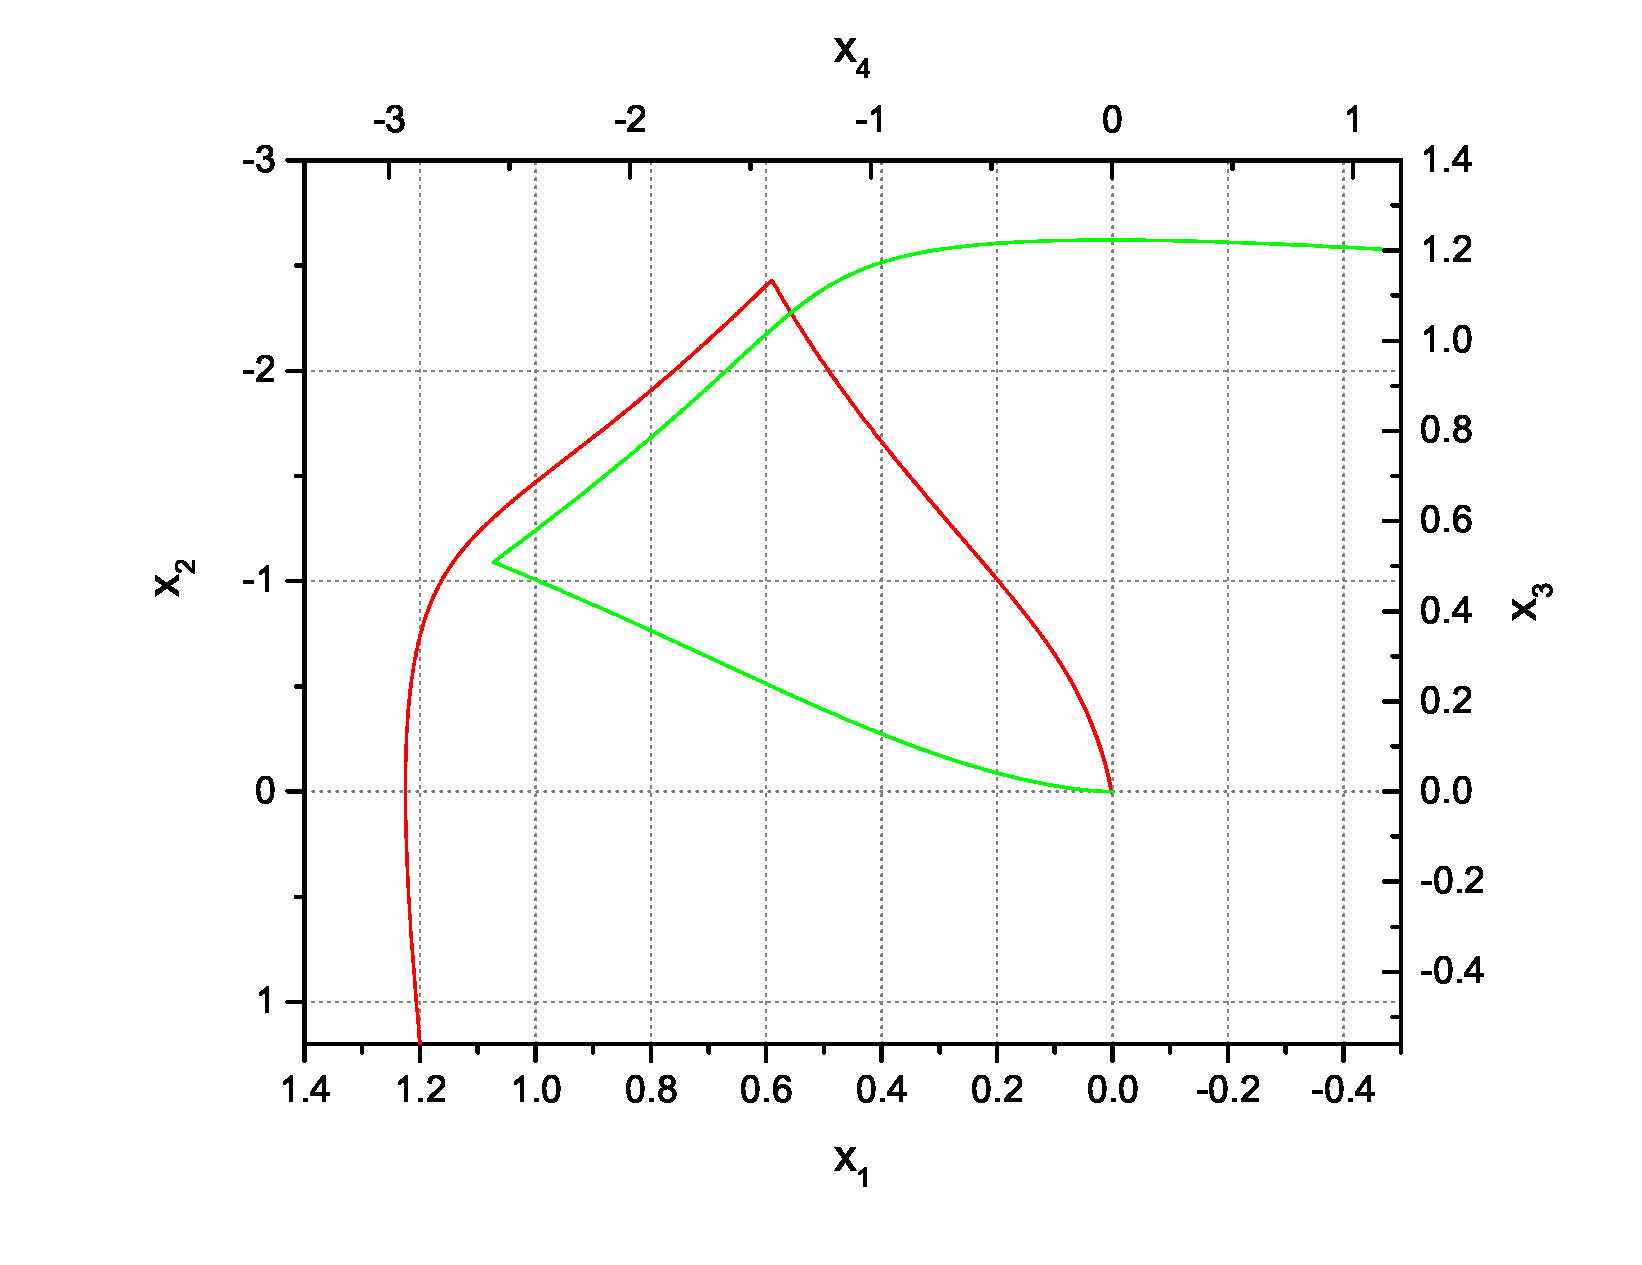
\includegraphics[width=0.7\textwidth]{paper3_fig2.eps}
\caption{Phase space trajectory}
\label{Figure:2}
\end{figure}

\begin{figure}[http]
\centering
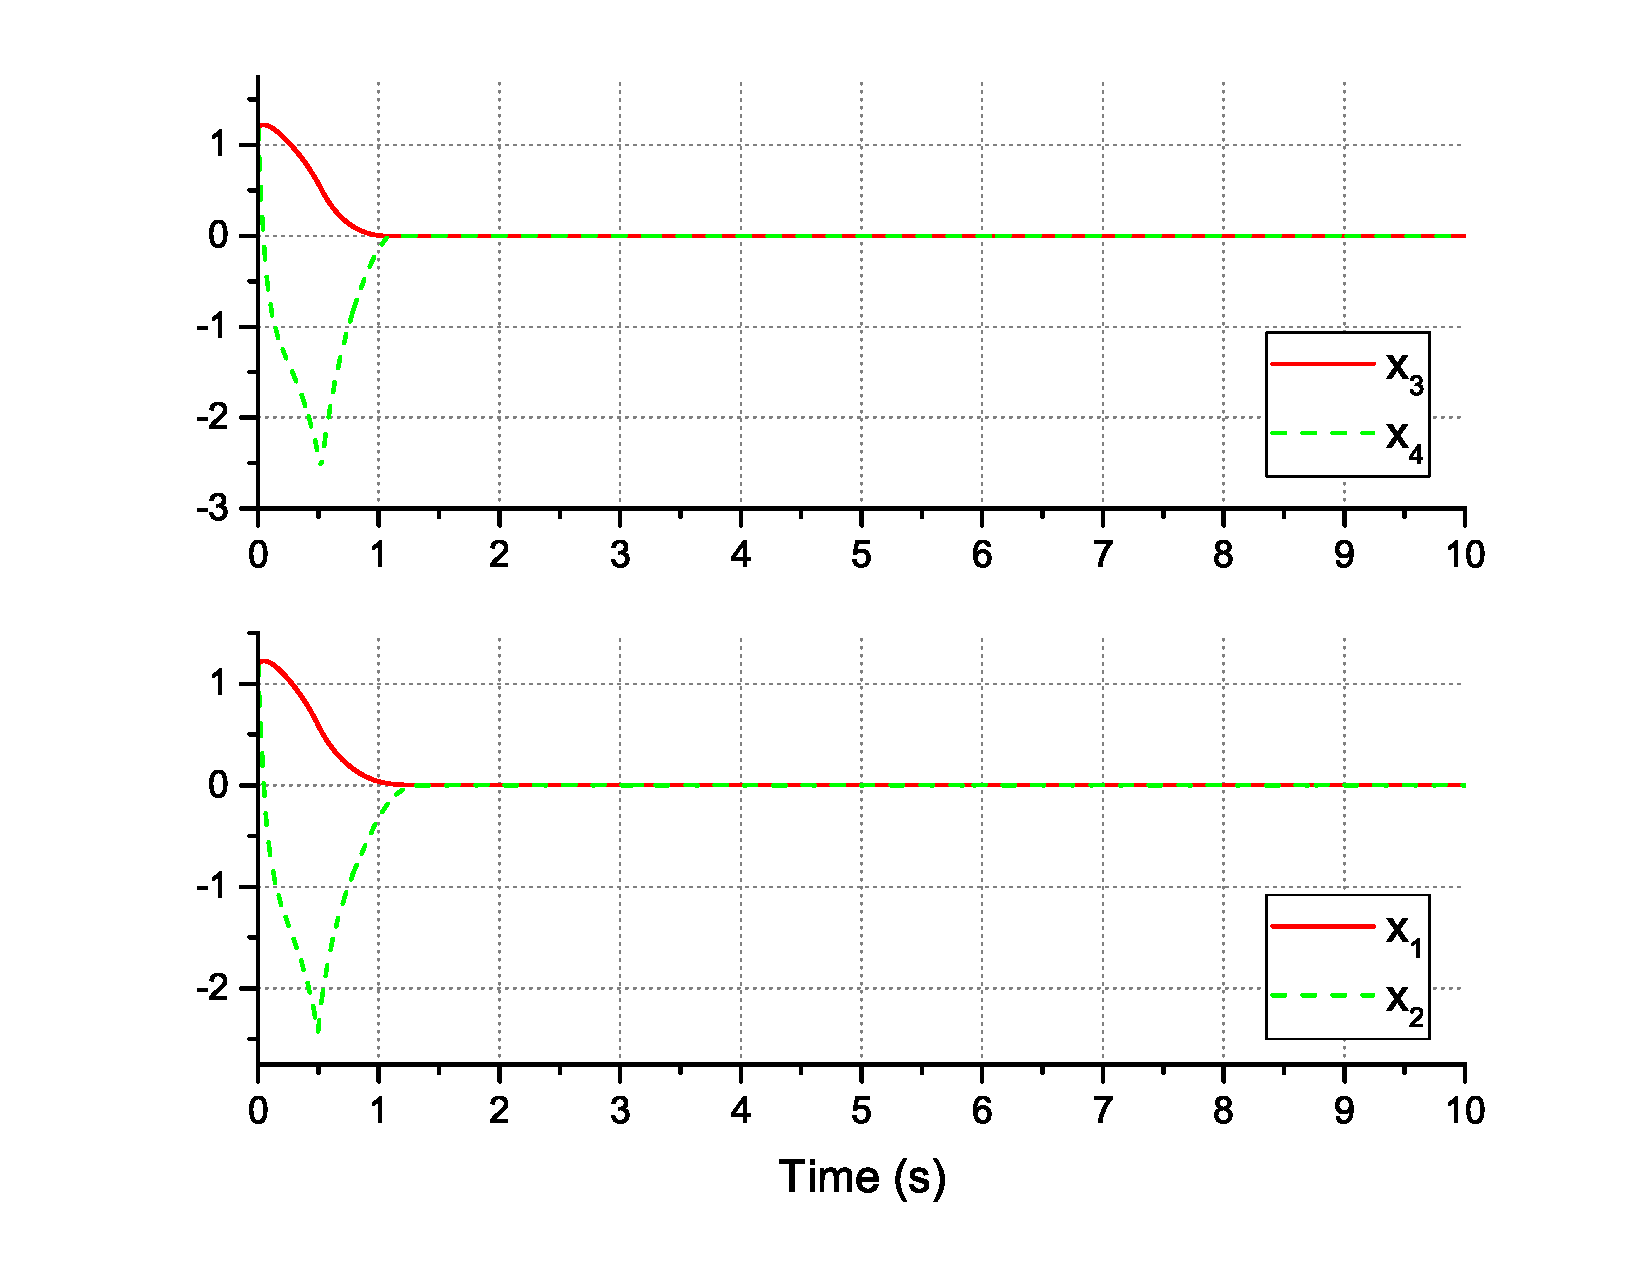
\includegraphics[width=0.7\textwidth]{paper3_fig2_20161108.eps}
\caption{system response}
\label{Figure:2_20161108}
\end{figure}

\begin{figure}[http]
\centering
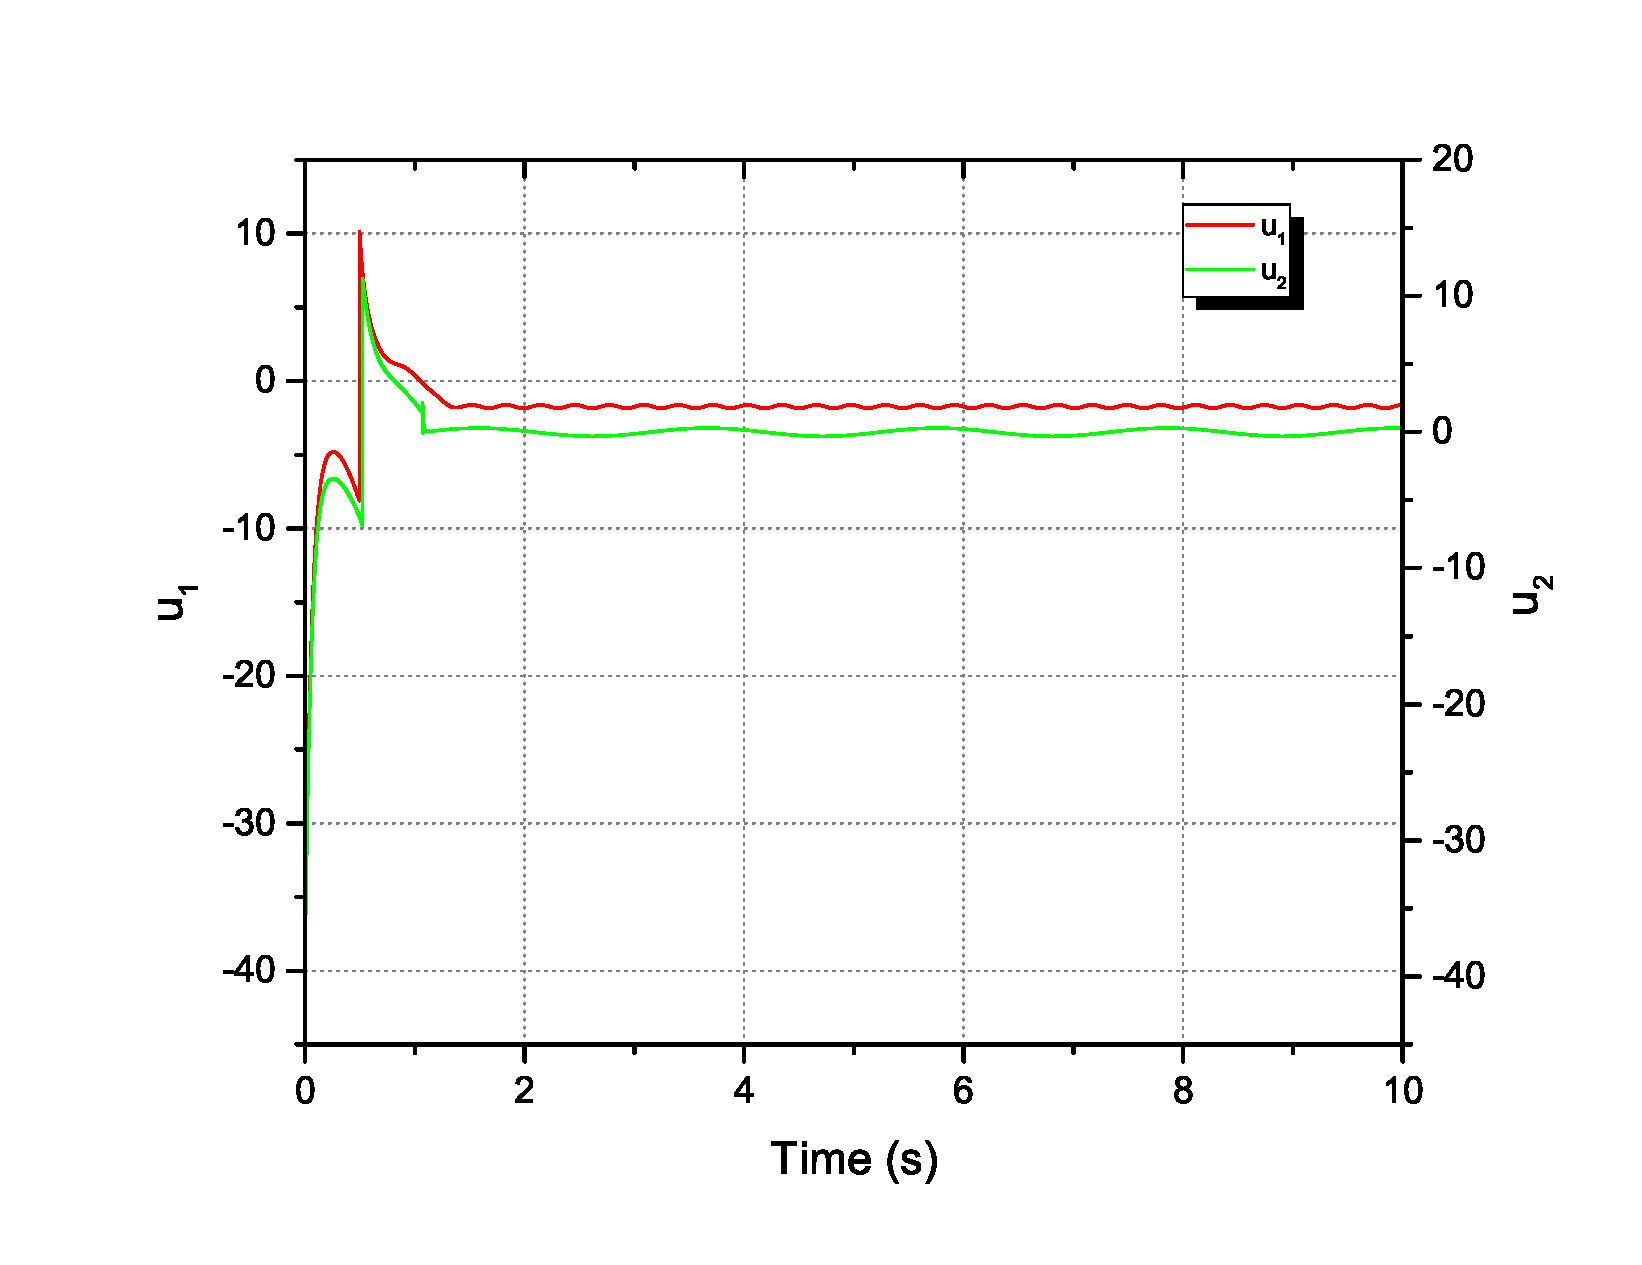
\includegraphics[width=0.7\textwidth]{paper3_fig3.eps}
\caption{System inputs}
\label{Figure:3}
\end{figure}
\begin{figure}[http]
\centering
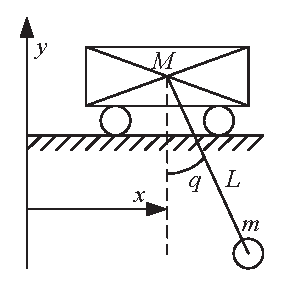
\includegraphics[width=0.3\textwidth]{paper3_fig8.eps}
\caption{Overhead crane schematic}
\label{Figure:8}
\end{figure}
\subsection{Underactuated example}
Figure~\ref{Figure:8} shows an overhead crane system, the state space equation of which is same with the formula in Eq.~(\ref{eq:underactuated system}) with state variables selected as $\bm x=(x,\dot x,q,\dot q)$, and the details are listed:
\begin{align}
\begin{split}
f_1&=(M+m\sin^2q)^{-1}(mL\dot q^2\sin q+mg\sin q\cos q)\\
b_1&=(M+m\sin^2q)^{-1}\\
f_2&=-(ML+mL\sin^2q)^{-1}((M+m)g\sin q+mL\dot q^2\sin q\cos q)\\
b_2&=-(ML+mL\sin^2q)^{-1}\cos q,
\end{split}
\end{align}
where $x$ is defined as the displacement of the horizontal direction, and $q$ stands for the swing angle from the vertical line. $M=1kg$ and $m=0.8kg$ donate the masses of the trolley and the load in Figure~\ref{Figure:8}, respectively, and $g=9.8m/s^2$ refers to as the acceleration of gravity. $L=0.305m$ represents the length of the rope. In this simulation, the disturbances are also introduced:
\begin{align}
g_1(\bm x)&= 0.02\sin t\\
g_2(\bm x)&=0.07e^{-4t},
\end{align}
and those boundaries are easy to obtain. The initial condition of the overhead crane system is $\bm x_0 = (0.1,0,0.1,0)$, while the desired status is $\bm x_d = (2,0,0,0)$. The HDSM controller can be designed with the following set of parameters:
$c_1=1$, $c_2=4$, $\eta_u = 0.1$, $k_u=1$, $\gamma = 1$, $\lambda = 3$, $\alpha = 0.6$.\par
Figure~\ref{Figure:9} shows the state response curves of the overhead crane system controlled using the HDSM control scheme, and the results show that the controller stabilize the displacement at $6s$ approximately, though the disturbance exists in the system. One can find that the swing angle is fluctuating in a fairly small range, the boundary of which is no more than $1\times 10^-3rad$, and this phenomena is reasonable and also occurs in the stable hierarchical SMC scheme~\cite{wang2004design}.
\begin{figure}[http]
\centering
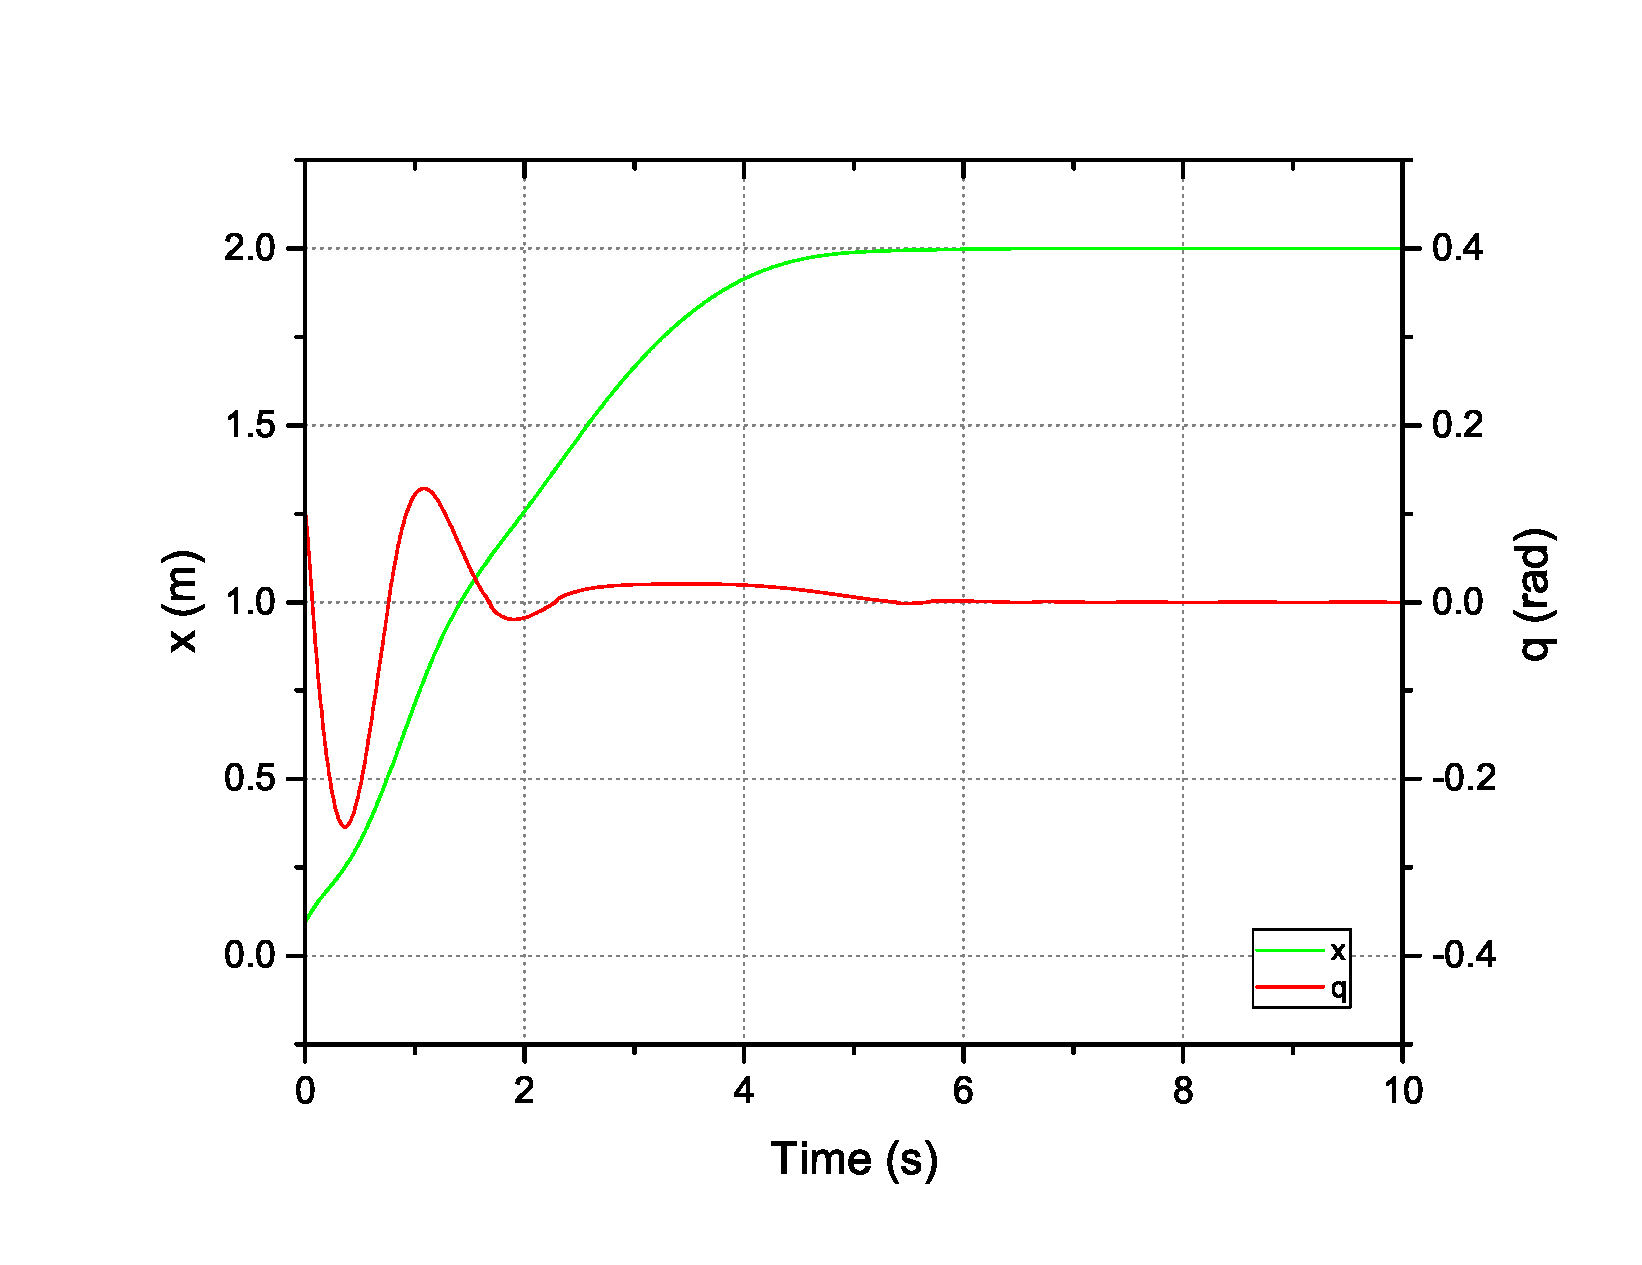
\includegraphics[width=0.7\textwidth]{paper3_fig9.eps}
\caption{Overhead crane dynamics}
\label{Figure:9}
\end{figure}
\subsection{Performance of the robotic manipulator}\label{sec:robotica manipulator}
In order to evaluate the performance of the proposed control scheme, a simulation about the $2$-link robotic manipulator is presented in the following context. Figure~\ref{Figure:1} is the $2$-link manipulator schematic, the dynamics of which can be explained by the dynamic equations in following forms:
\begin{figure}[http]
\centering
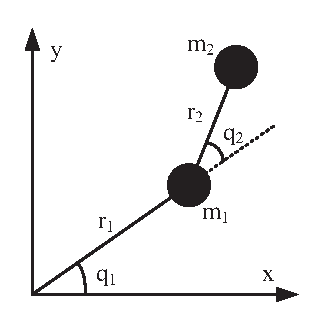
\includegraphics[width=0.3\textwidth]{paper3_fig1.eps}
\caption{$2$-link manipulator schematic}
\label{Figure:1}
\end{figure}

\begin{align}
\begin{bmatrix}
m_{12}(q_2) &m_{12}(q_2)\\
m_{21}(q_2) &m_{22}
\end{bmatrix}
\begin{pmatrix}
\ddot q_1\\
\ddot q_2
\end{pmatrix}
+
\begin{bmatrix}
-c(q_2)\dot q_1^2-2c(q_2)\dot q_1\dot q_2\\
c(q_2)\dot q_2^2
\end{bmatrix}+
\begin{bmatrix}
\xi_1(q_1,q_2) g\\
\xi_2(q_1,q_2) g
\end{bmatrix}=
\begin{pmatrix}
\tau_1\\
\tau_2
\end{pmatrix},\label{eq:manipulator}
\end{align}
where
\begin{align*}
&m_{11}(q_2)=(m_1+m_2)r_1^2+m_2r_2^2+2m_2r_1r_2\cos(q_2)+J_1,\\
&m_{12}(q_2)=m_2r_2^2+m_2r_1r_2\cos(q_2),\\
&m_{21}(q_2)=m_{12}(q_2),\\
&m_{22}=m_2r_2^2+J_2,\\
&c(q_2)=m_2r_1r_2\sin(q_2),\\
&\xi_1(q_1,q_2) =(m_1+m_2)r_1\cos(q_2)+m_2r_2\cos(q_1+q_2),\\
&\xi_2(q_1,q_2) = m_2r_2\cos(q_1+q_2).
\end{align*}\par
The values of the parameters are listed here, $r_1=1m$, $r_2=0.8m$, $J_1=5 kgm$, $J_2=5kgm$, $m_1=0.5kg$, $m_2=1.5kg$. In this model, the uncertainty is brought in by estimated terms, namely, $\bar m_1=0.4$ and $\bar m_2=1.2$ which are all not the actual value obviously. Accordingly, the uncertainty parameters in Eq.~(\ref{eq:manipulator uncertainty}) are assumed to be $\mu_0=10$, $\mu_1=3$, $\mu_2=3$.

This section will give a set of simulation to examine the step response performance of the MDTSM controller. The behavior of the manipulator should fulfill the initial and desired conditions, namely, $(\bm q_0^T, \dot{\bm q}_0^T)= (0.3,0.2,0,0)$ and $({\bm q}_d^T,\dot{\bm q}_d^T)=(1,1,0,0)$. In order to ensure the stability and the fast convergence speed, the control parameters are chosen conservatively to make the manipulator stable in finite time, and these parameters are $\alpha = 0.6$, $\gamma = 1$, $\lambda = 0.1$, $k = 150$. The TSM controller, as a comparison, is also implemented to regulate the behavior of the manipulator:
\begin{align}
\begin{split}
\bm s &= \dot{\bm \varepsilon}+C_\gamma\lceil\bm{sgn}^\alpha(\bm \varepsilon)\rfloor\\
\bm\tau &= \bm u_0+\bm u_1 +\bm u_2\\
\bm u_0 &= -M_0(\bm q)C_r\lceil\alpha\vert\bm\varepsilon\vert^{\alpha-1}\dot{\bm \varepsilon}\rfloor\\
\bm u_1 &= M_0(\bm q)\ddot {\bm q}_d+C_0(\bm q,\dot {\bm q})+g_0(\bm q)\\
\bm u_2 &= -k\frac{(\bm s^TM_0^{-1}(\bm q))^T}{\Vert\bm s^TM_0^{-1}(\bm q)\Vert}.
\end{split}
\end{align}
where the main control parameters of which are selected as $\alpha = 0.6$, $\gamma = 5$ and $k = 150$ to get a fairly good control performance.

\begin{figure}[http]
\centering
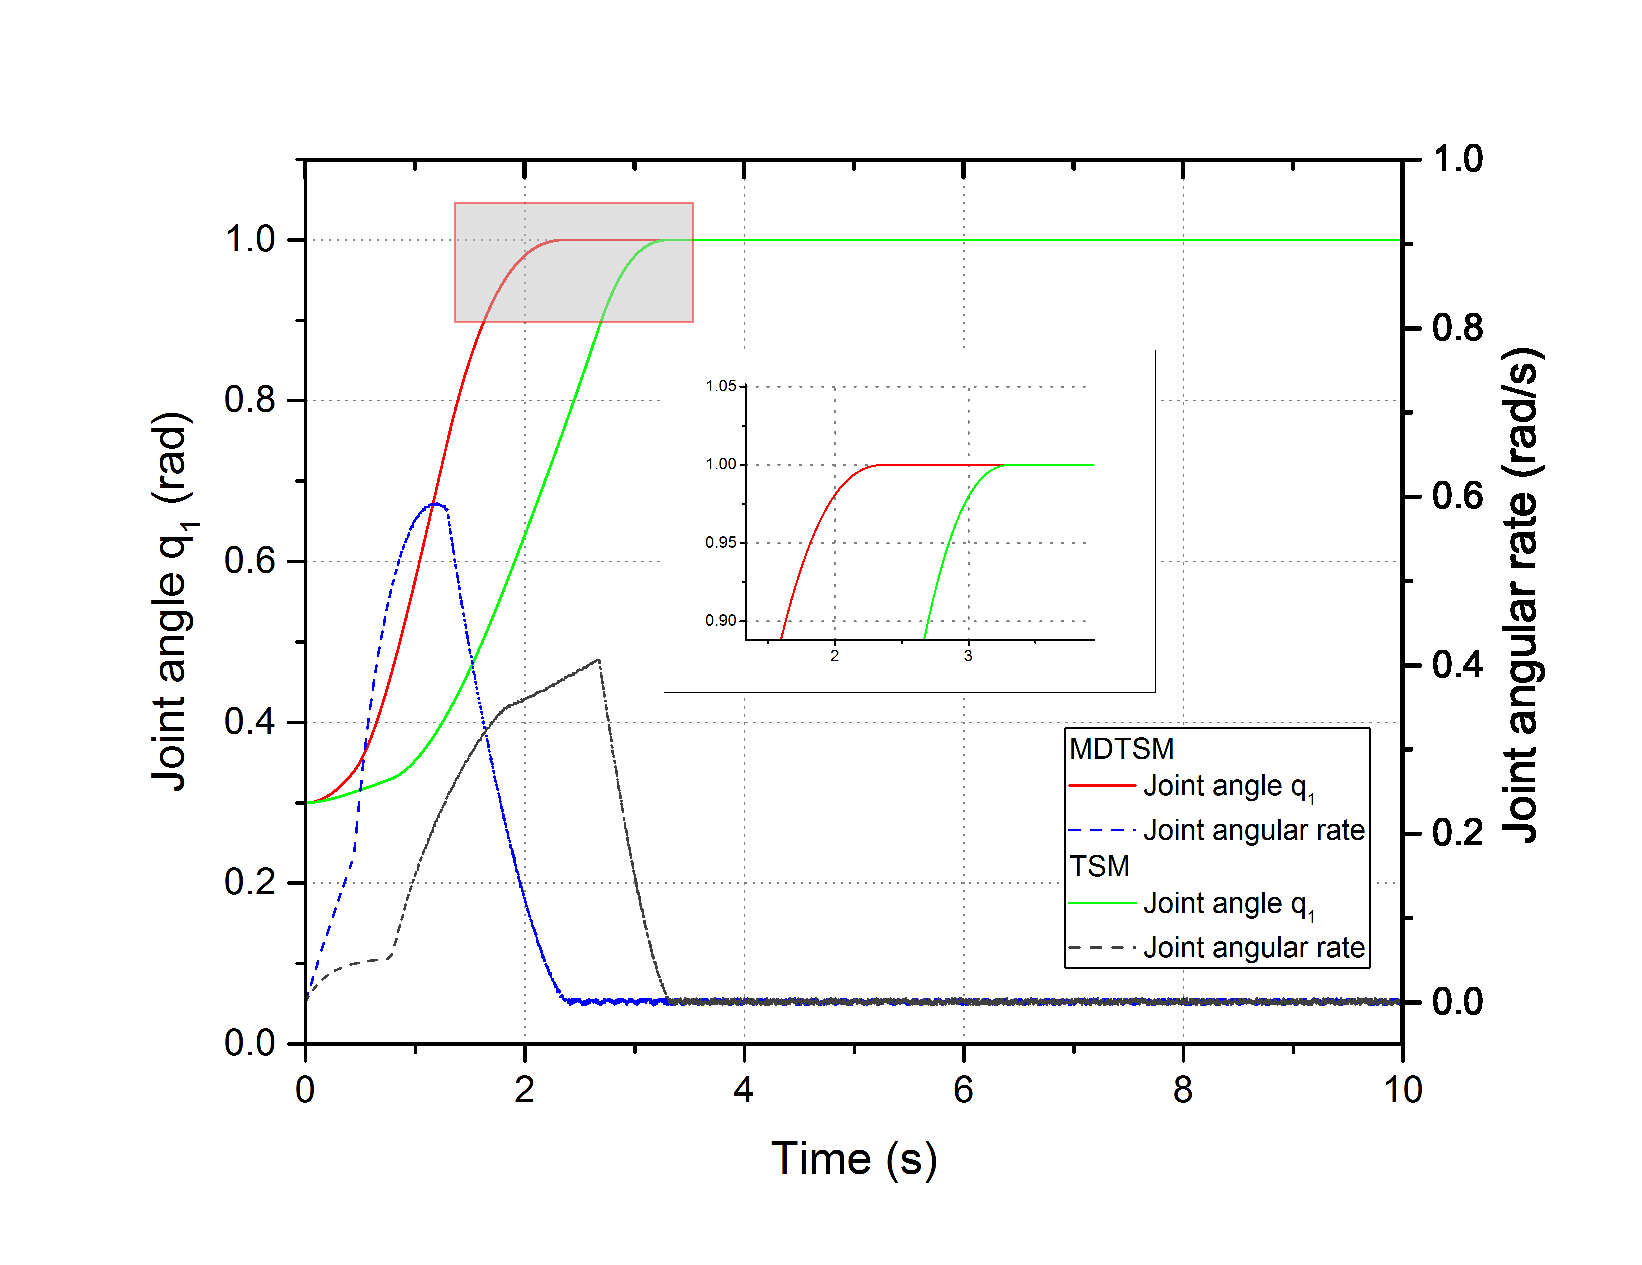
\includegraphics[width=0.7\textwidth]{paper3_fig4.eps}
\caption{Response of $q_1$ channel}
\label{Figure:4}
\end{figure}

\begin{figure}[http]
\centering
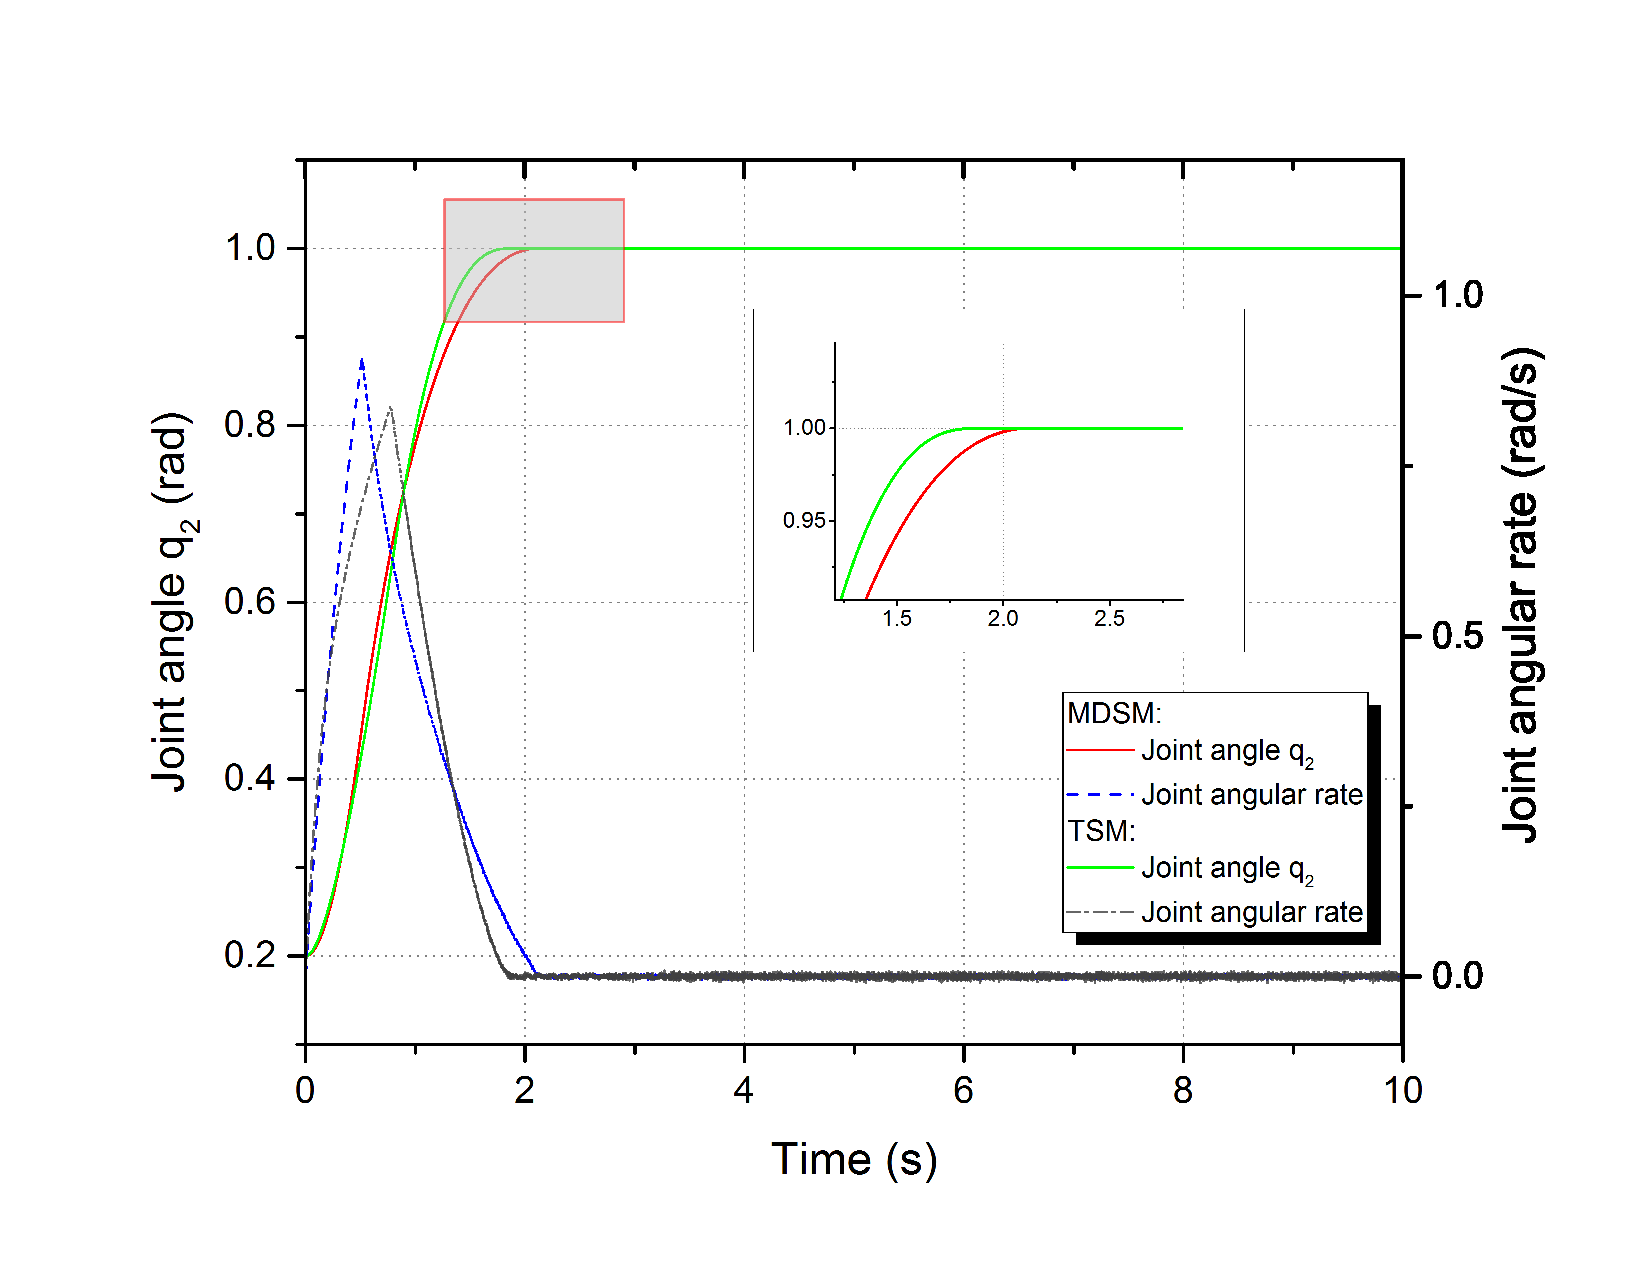
\includegraphics[width=0.7\textwidth]{paper3_fig5.eps}
\caption{Response of $q_2$ channel}
\label{Figure:5}
\end{figure}

\begin{figure}[http]
\centering
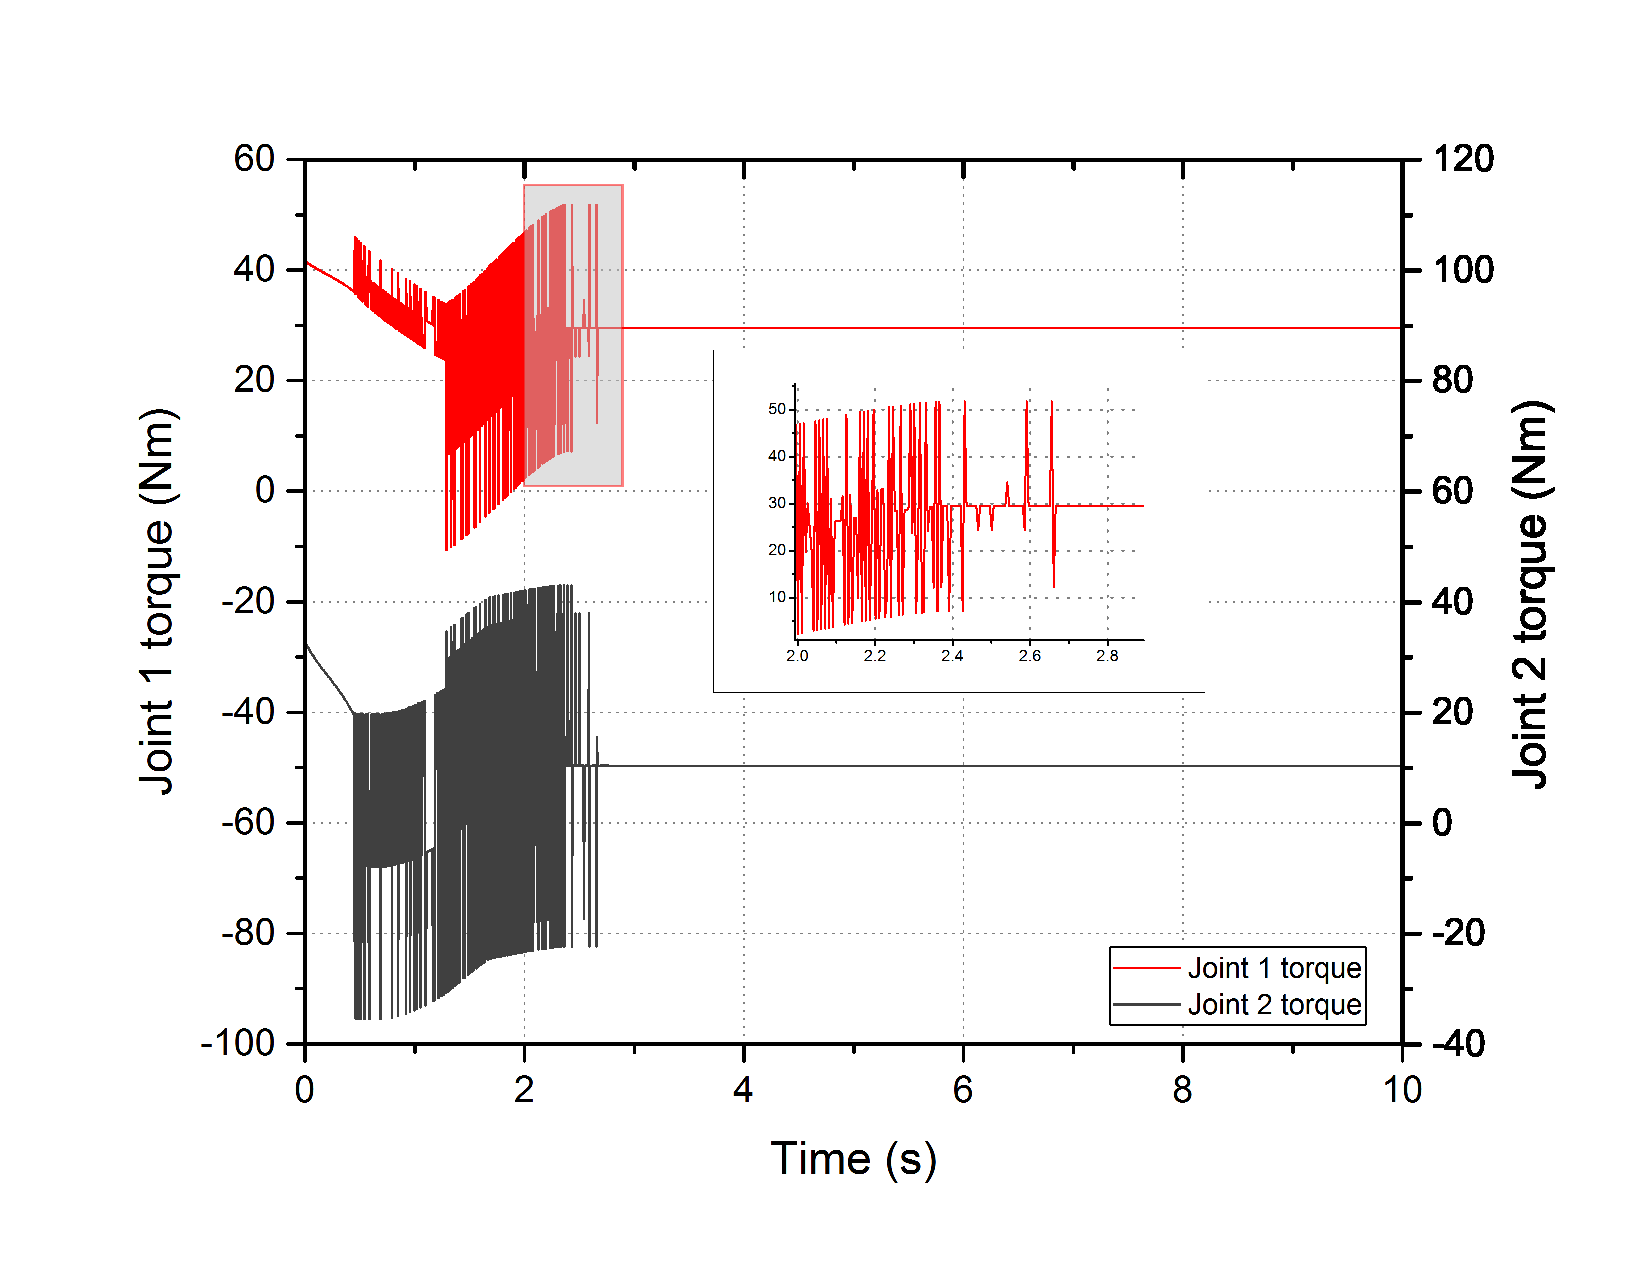
\includegraphics[width=0.7\textwidth]{paper3_torque.eps}
\caption{Joint torques}
\label{Figure:torque}
\end{figure}
The performance of the controllers mentioned above is illustrated in Figure~\ref{Figure:4} and Figure~\ref{Figure:5}. \textcolor{red}{For the MDTSM controller, the joint~1 finishes its desired behaviour at about $2.3s$, and meanwhile the joint~2 spends about $1.7s$ completing the desired mission. Also, by observing the results, we can find that the stabilization time of the proposed method is less than the TSM controller's, and the regulating process of the manipulators is steady and reasonable. Through calculation, we can find the maximum theoretical finite convergence time $t_f=3.0843s$, which can be obtained directly according to Eq.~(\ref{eq:total convergence time}) and simulation data, is more than $2.3s$, the convergence time of the simulation result. Hence, we can conclude that the results have verified the analyses about the convergence time in Section~\ref{sec:2}.  The control torques of the joints are depicted in Figure~\ref{Figure:torque}. It is obvious that the torques of the two joints are both switching dramatically at the beginning, and this phenomenon is caused directly by the rapidly changing sliding mode dynamics $s_i$. Moreover, at about $1.7s$, all the joint states are regulated to locate in the vicinity of the origin, but the sliding mode dynamics do not yet enter the boundary layer $s_i< \delta$. This switching inputs last about $2.7s$ before reaching the boundary layer. After $2.7s$ boundary layer technique works to generate continuous torques, which maintain a reasonable constant in the subsequent time, since the overall system has been stable.} Therefore these results show that the MDTSM control scheme can achieve the regulation of the manipulator effectively.

\textcolor{red}{At this point, we have verified the feasibility of the MDTSM controller on step responses of the joints of the manipulator, and in most engineering applications, manipulators are required to track the variable desired signals, which own the actual physical meanings, such as polish, machine tools and laser beam cutting. Accordingly, the tracking performance of the robotic manipulator controlled by the proposed methods is studied in this section, and we continue to use the parameters of the controller mentioned above, and the mission condition is changed as follows:}
\begin{align*}
&(\bm q_0^T, \dot{\bm q}_0^T)= (1.5,1.5,0,0)\\
&{\bm q}_d^T=(1.25-(1/5)e^{-t}+(1/20)e^{-4t},1.25+(9/40)e^{-t}-(1/4)e^{-2t})
\end{align*}\par
 \textcolor{red}{The simulation results are demonstrated in Figure~\ref{Figure:6} and Figure~\ref{Figure:7}, which plot the trajectories of joints of the manipulator~(\ref{eq:manipulator}) regulated by adopting the MDTSM controller. In Figure~\ref{Figure:6}, the tracking error between the variable desired signal and the joint angle $q_1$ keeps decreasing from the initial status, and the two trajectories reach a confluence at about $3s$, which means that $q_1$ has absolutely tracked the variable desired signal. The similar conclusion about $q_2$ can also be obtained from the results in Figure~\ref{Figure:7}. From the enlarged figures, we can detect that the controller perform the high-precision tracking due to the completely coincident curves after $3s$. In addition, the great slopes of the tangent the tracking curves guarantee that the curves can converge to the desired signal curves in short time, and also lead to small overshoot in joint~1 angle regulation, which is reasonable and does not affect the tracking performance in the subsequent time. Taken as a whole, the control system completes the tracking mission at about $3.2s$ from the prescript initial conditions, which performs the smoothly tracking motion subjected to the variable desired signals.}
\begin{figure}[http]
\centering
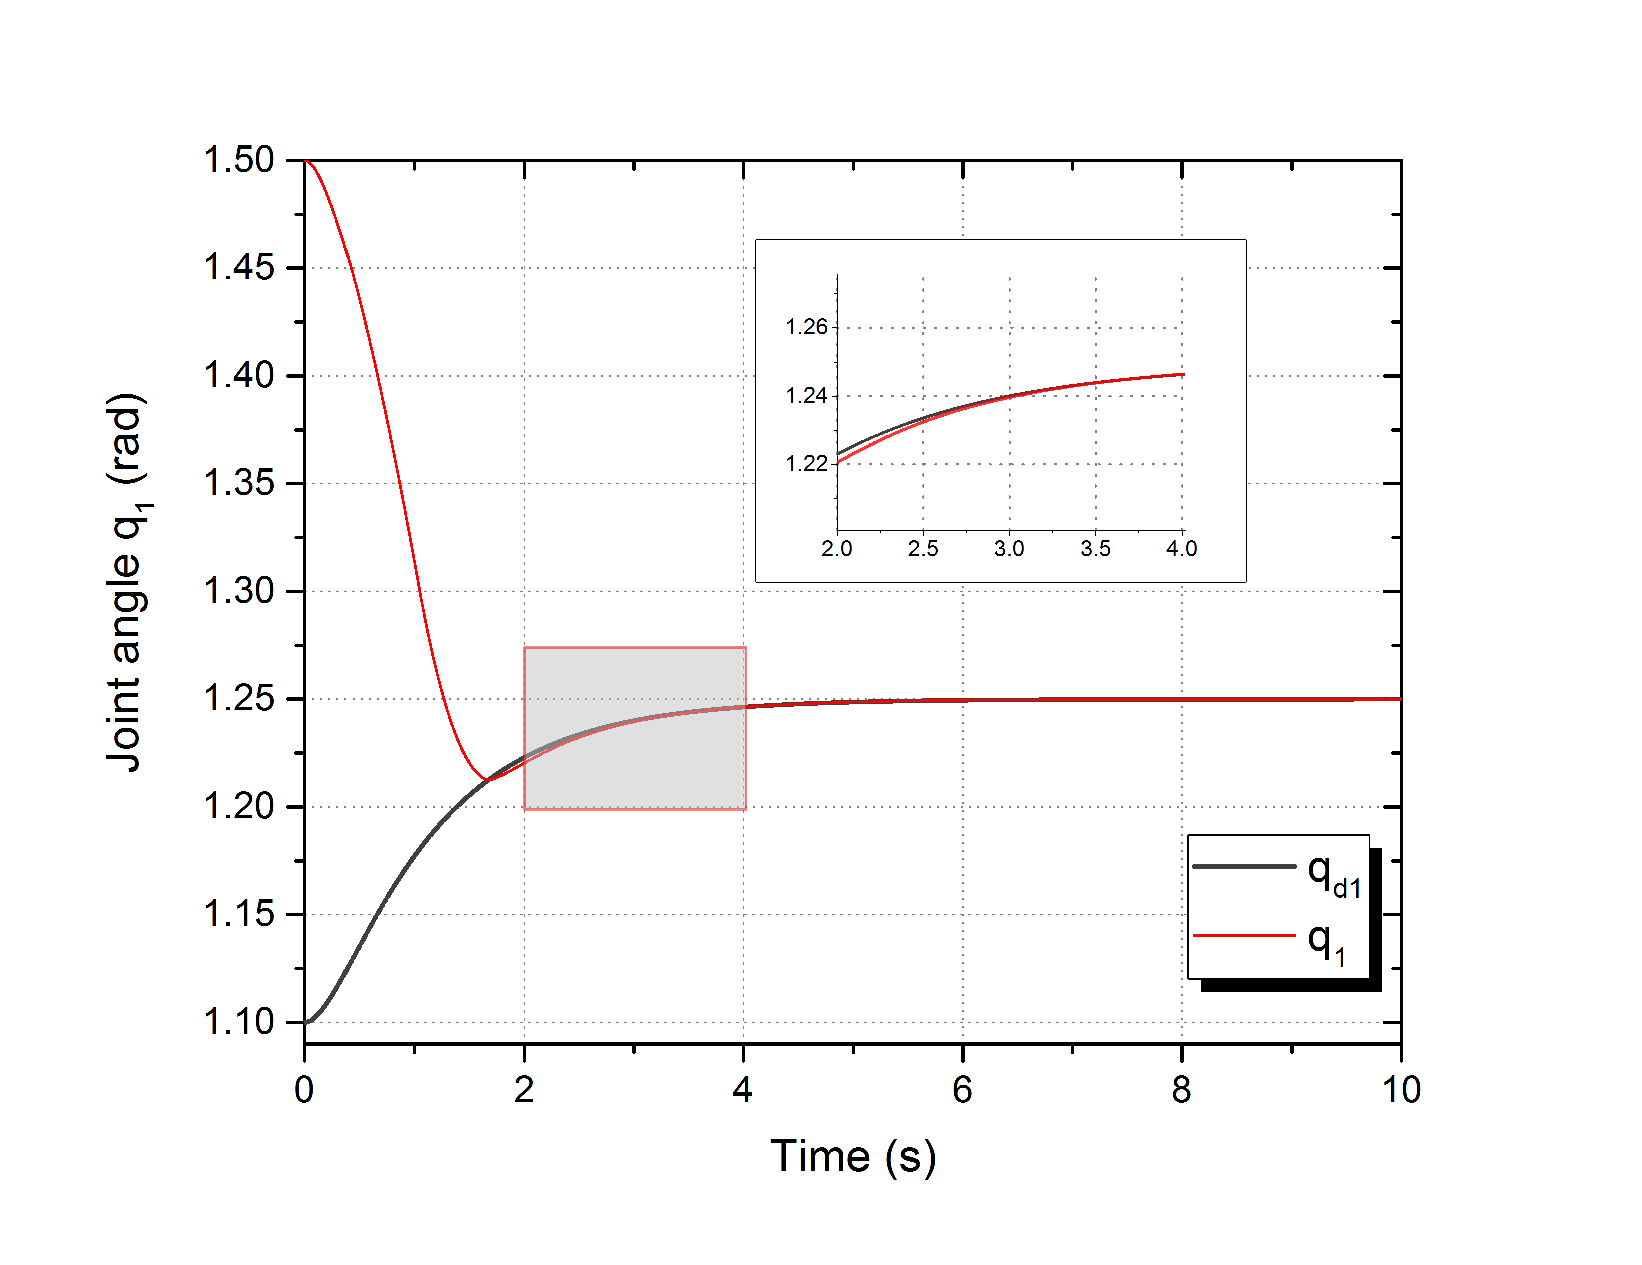
\includegraphics[width=0.7\textwidth]{paper3_fig6.eps}
\caption{Tracking performance of $q_1$ channel}
\label{Figure:6}
\end{figure}

\begin{figure}[http]
\centering
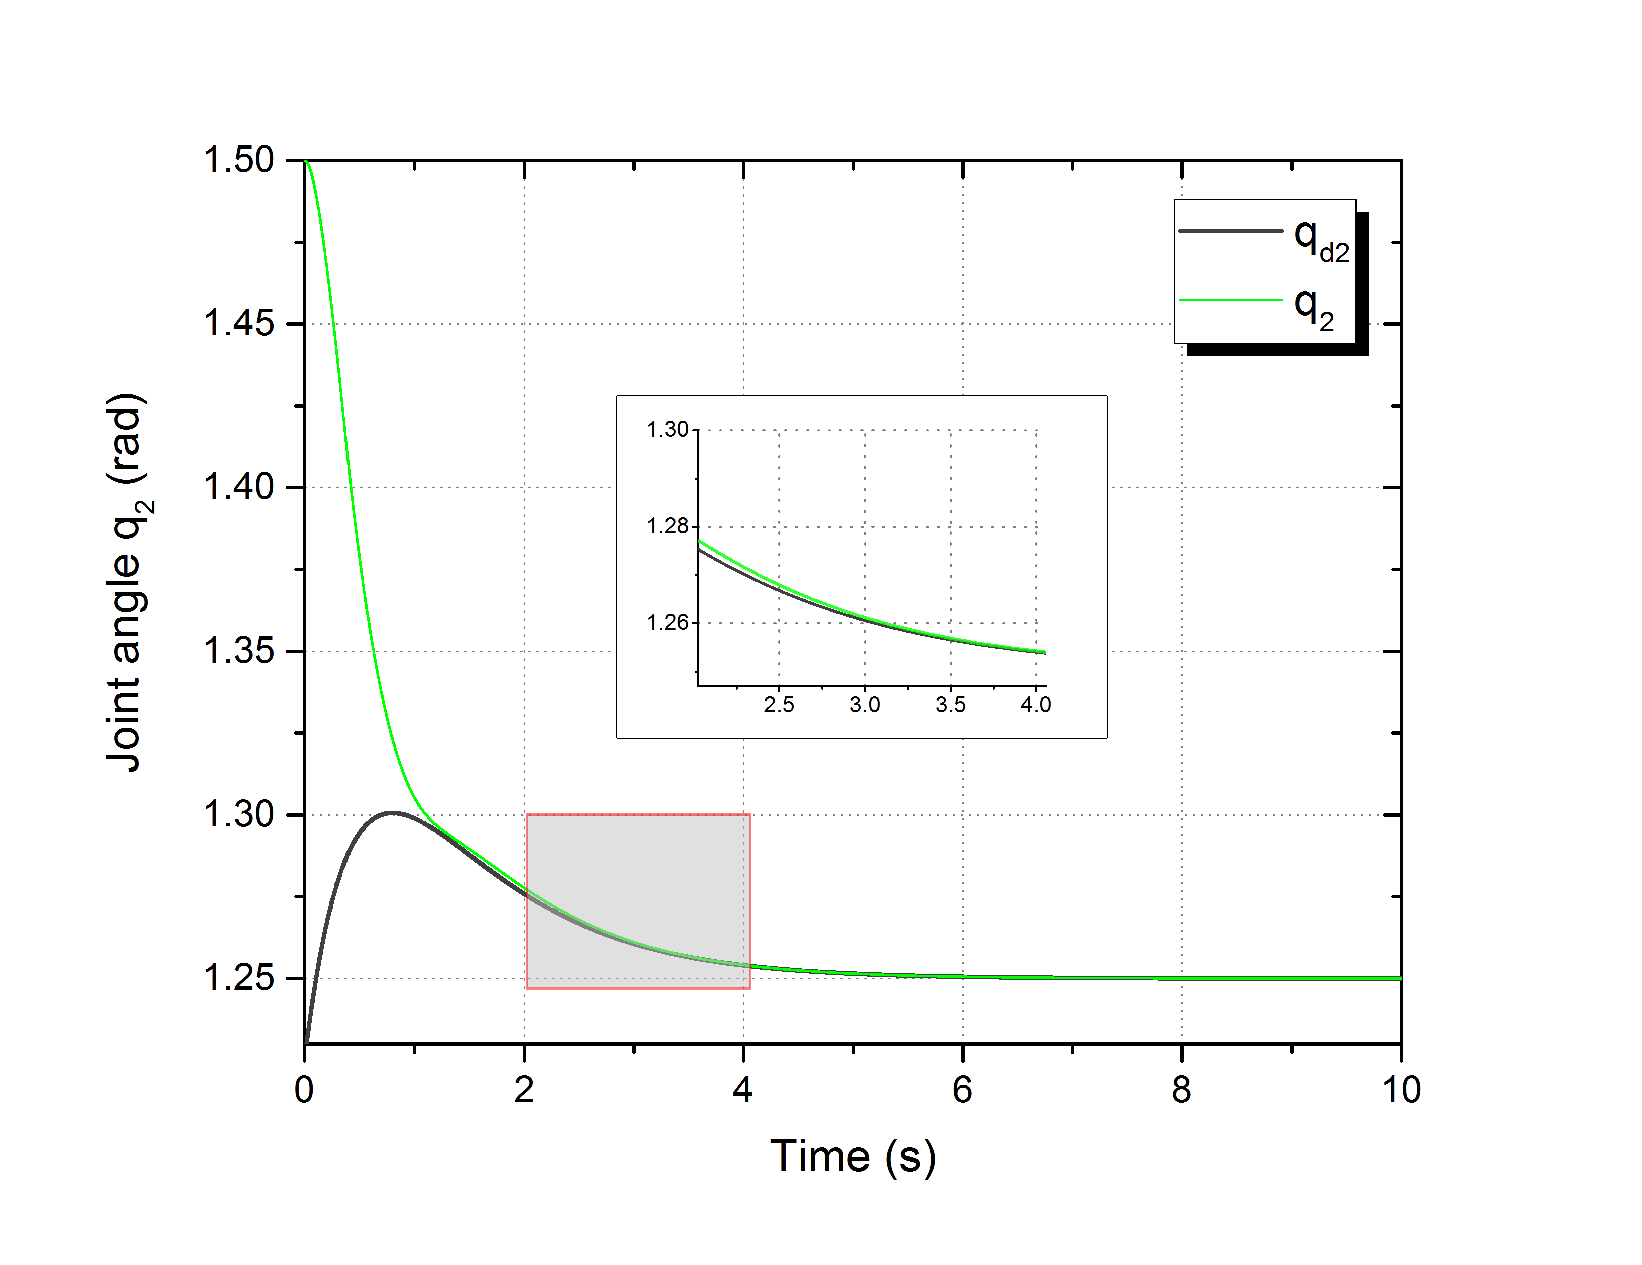
\includegraphics[width=0.7\textwidth]{paper3_fig7.eps}
\caption{Tracking performance of $q_2$ channel}
\label{Figure:7}
\end{figure}
\textcolor{red}{Another important issue that we always meet in engineering applications, is the actuator constraint due to the physical limitation, which can be regarded as the input limitation problem shown in Eq.~(\ref{eq:second-order system subjected to limitation}). Consider the case that there exists the input limitation in the manipulator model~(\ref{eq:manipulator}), and without loss of generality, the maximum torque of the joint is $50Nm$. Reviewing the torque curve of joint~1  shown in enlarged details of  Figure~\ref{Figure:torque}, we can find that the torque exceeds the reasonable torque upper limit $50Nm$ around $2.3s$. If we still use the MDTSM controller to stabilize the system subjected to input limitation, we can not get the same results as shown in Figure~\ref{Figure:torque}, and this is because that the limitation hamper the rigorous theoretical analyses of Theorem~\ref{theorem:2}. Hence, to overcome this issue, the adaptive MDTSM controller is applied to diminish the effect of the input limitation and to guarantee the rigorous stability analyses.}
\begin{figure}
\centering
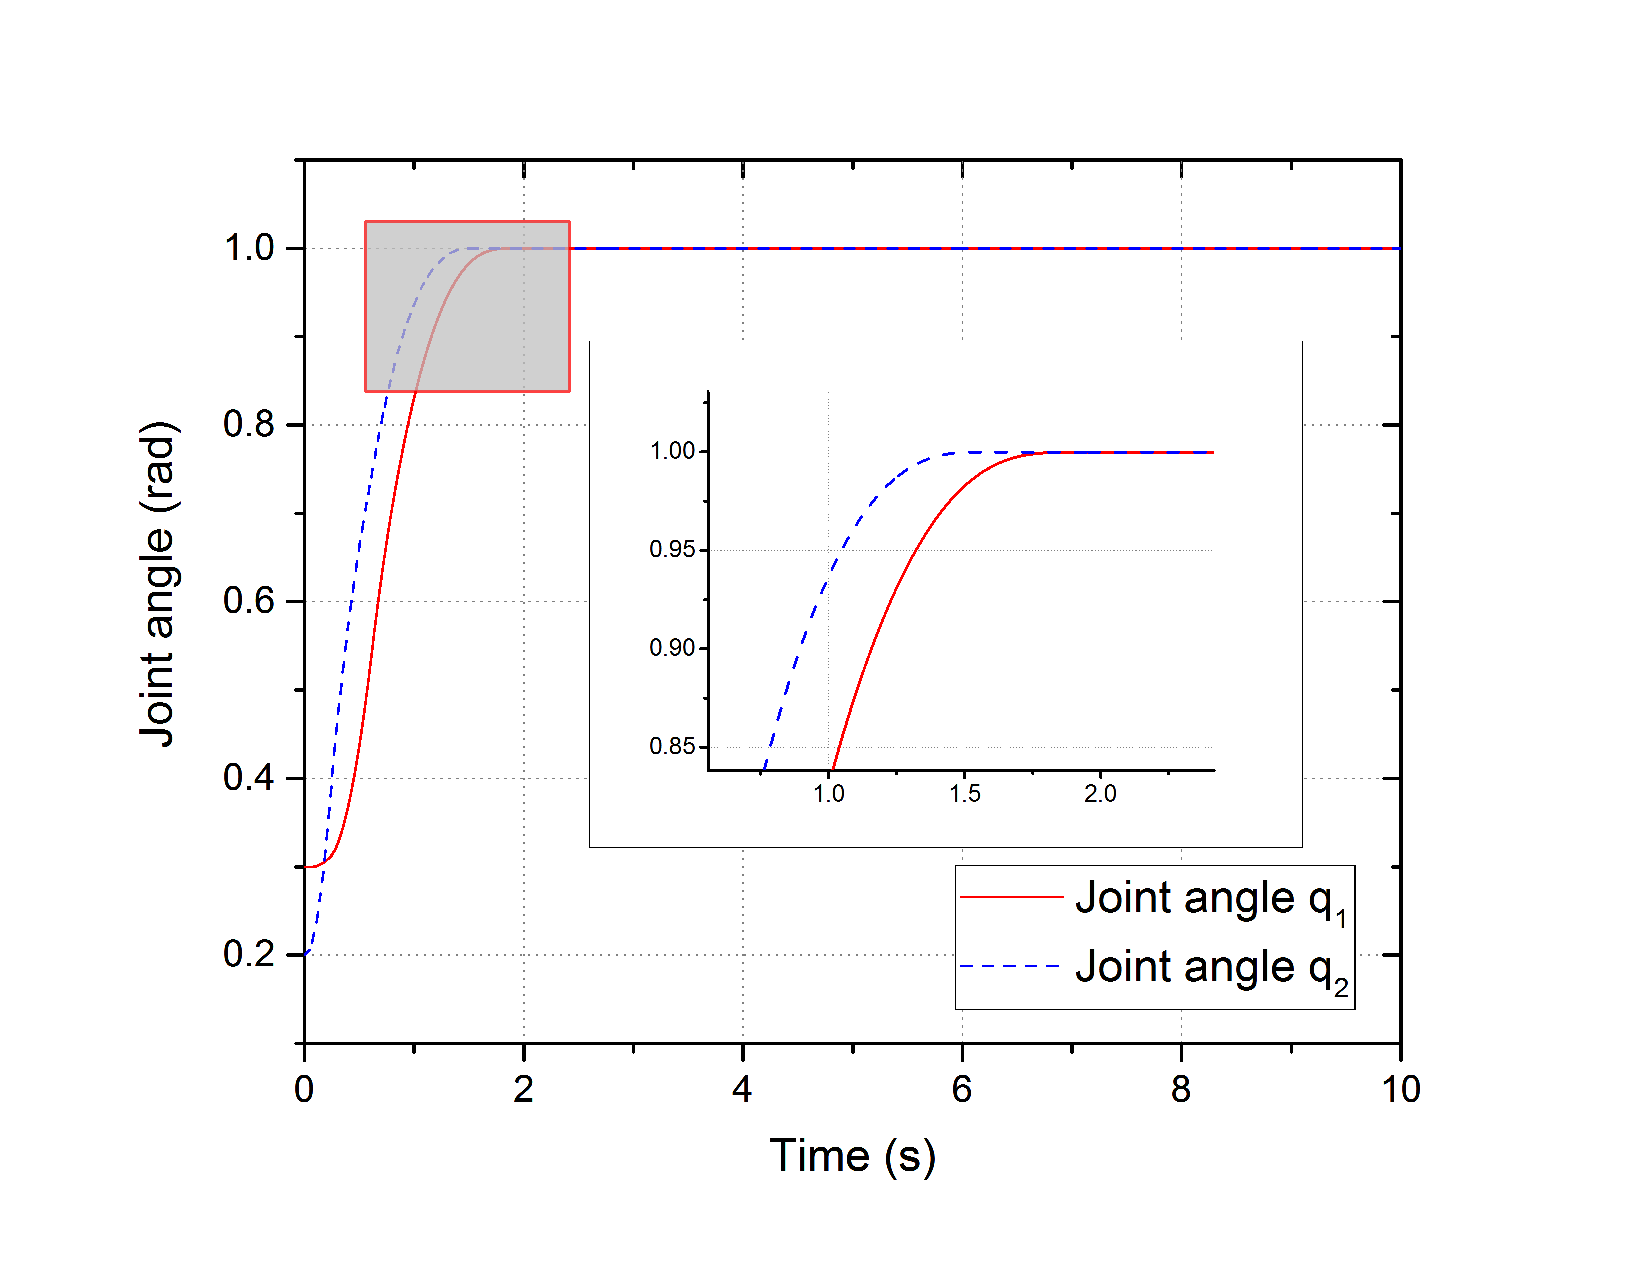
\includegraphics[width=0.7\textwidth]{paper3_fig_limitation_q.eps}
\caption{Trajectories of manipulator dynamics subjected to input limitation}
\label{Figure:limitation_q}
\end{figure}
\begin{figure}
\centering
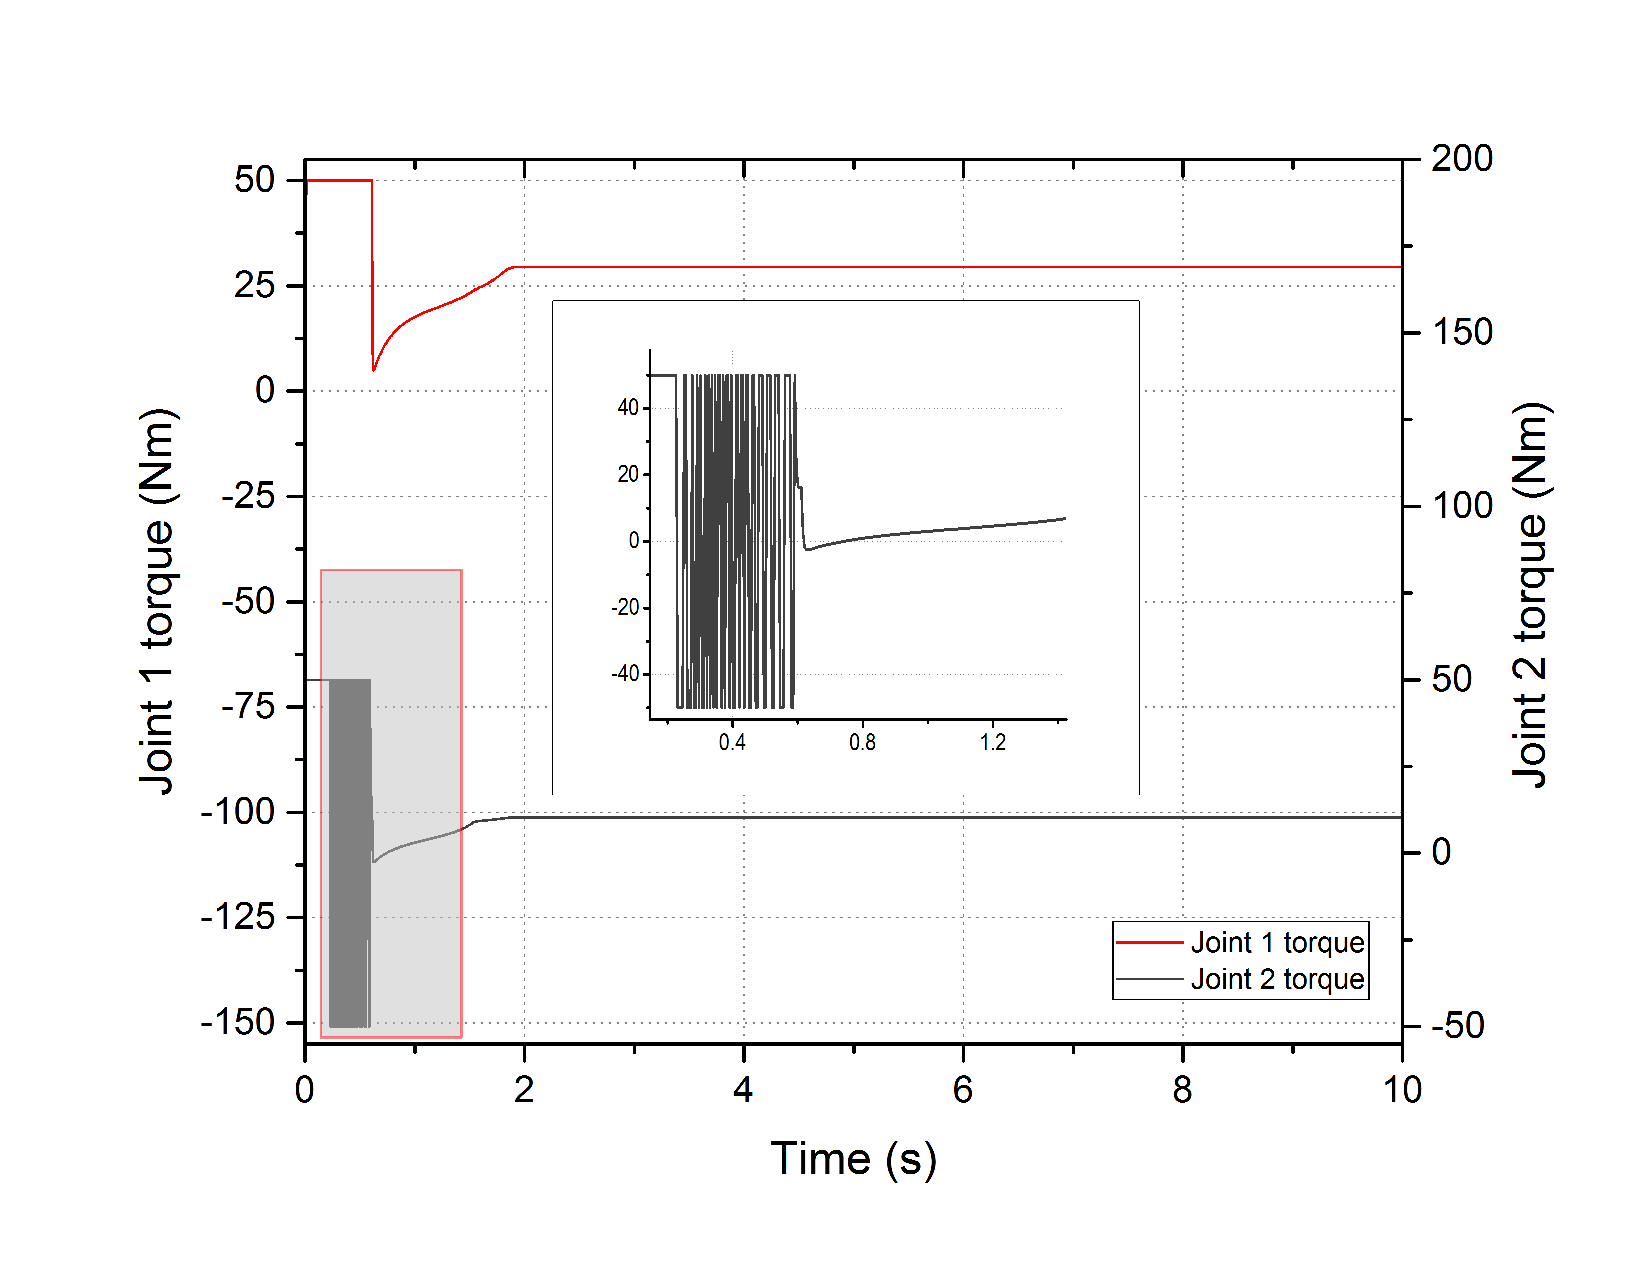
\includegraphics[width=0.7\textwidth]{paper3_fig_limitation_torque.eps}
\caption{Trajectories of joint torques subjected to  input limitation}
\label{Figure:limitation_torque}
\end{figure}
\textcolor{red}{Here we examine the step response of the adaptive MDTSM control scheme for the robotic manipulator dynamics, since the step response is a severe challenge to the controller. Accordingly, the initial and desired conditions are $(\bm q_0^T, \dot{\bm q}_0^T)= (0.3,0.2,0,0)$ and $({\bm q}_d^T,\dot{\bm q}_d^T)=(1,1,0,0)$, respectively. The design parameters of the adaptive MDTSM controller can be selected as $\varpi_1=50$, $\varpi_2=30$, $\varphi_1=\varphi_2=0.01$, $\nu_1 = 5$, $\nu_2=6$, $\omega_1=\omega_2=1$ to satisfy the parameter conditions in Theorem~\ref{thm:4}. In addition, for better tracking performance, the boundary layer thickness is revised as $\delta=0.1$. }

\textcolor{red}{The results shown in Figure~\ref{Figure:limitation_torque} indicate that the joint torques are limited in the region $[-50,50]Nm$ from $0s$ to $0.4s$, while the trajectories in the Figure~\ref{Figure:limitation_q} demonstrates that the manipulator dynamics are still under control. The limitations occur in the beginning stage of the regulation, since the large tracking errors lead to the great command inputs. Moveover the boundary layer technique works after $0.4s$ and generates continuous torques in the subsequent time. Compared to the results in Figure~\ref{Figure:torque}, we can find that the boundary layer of the adaptive MDTSM controller functions earlier, and this is because that the thickness is modified as $\delta=1\times 10^{-1}$ from $\delta=1\times 10^{-4}$. It implies that $s_i<\delta$ appears earlier for the adaptive MDTSM controller than the MDTSM controller. Also, compared to the results from Figure~\ref{Figure:4}, we can find that the rise time of the adaptive MDTSM controller is less, although the torques are limited strictly. Hence, we can conclude that the proposed adaptive MDTSM controller can regulate the robotic manipulator subjected to the input limitation, and the control performance is even better than the MDTSM controller for the system without input limitation in some extent.}
\section{Conclusion}\label{sec:5}
A feasible MDTSM control for n-link robotic manipulator has been presented. The method integrates two individual subsystems as a unity, then builds the surfaces and inputs for it to complete the controller design. The control scheme can guarantee the reaching condition of the desired sliding mode  surface, meanwhile the system states converge to the origin along the desired sliding mode  surface. Also, the entire convergence time can be calculated accordingly. Developing the basic DTSM yields the MDTSM controller, which provides a solution to eliminating chattering, avoiding singularity and fast convergence. For dealing with the underactuated characteristics which may appear in the system, the HDTSM control is derived, and the overhead crane example verifies its effectiveness. However, the control parameters selection is still a challenge especially in the HDTSM control scheme, and we will effort to excavate a full order dual TSM methodology in the future for removing the obstacle caused by parameters essentially.
\section{Acknowledgment}
This work is partially supported by the National Natural Science Foundation of China (No. 61104112, 61503101).
\section{References}
\bibliography{paper3_ref}
\bibliographystyle{elsarticle-num}
\end{document}
